\documentclass[twoside]{book}

% Packages required by doxygen
\usepackage{fixltx2e}
\usepackage{calc}
\usepackage{doxygen}
\usepackage[export]{adjustbox} % also loads graphicx
\usepackage{graphicx}
\usepackage[utf8]{inputenc}
\usepackage{makeidx}
\usepackage{multicol}
\usepackage{multirow}
\PassOptionsToPackage{warn}{textcomp}
\usepackage{textcomp}
\usepackage[nointegrals]{wasysym}
\usepackage[table]{xcolor}

% Font selection
\usepackage[T1]{fontenc}
\usepackage[scaled=.90]{helvet}
\usepackage{courier}
\usepackage{amssymb}
\usepackage{sectsty}
\renewcommand{\familydefault}{\sfdefault}
\allsectionsfont{%
  \fontseries{bc}\selectfont%
  \color{darkgray}%
}
\renewcommand{\DoxyLabelFont}{%
  \fontseries{bc}\selectfont%
  \color{darkgray}%
}
\newcommand{\+}{\discretionary{\mbox{\scriptsize$\hookleftarrow$}}{}{}}

% Page & text layout
\usepackage{geometry}
\geometry{%
  a4paper,%
  top=2.5cm,%
  bottom=2.5cm,%
  left=2.5cm,%
  right=2.5cm%
}
\tolerance=750
\hfuzz=15pt
\hbadness=750
\setlength{\emergencystretch}{15pt}
\setlength{\parindent}{0cm}
\setlength{\parskip}{0.2cm}
\makeatletter
\renewcommand{\paragraph}{%
  \@startsection{paragraph}{4}{0ex}{-1.0ex}{1.0ex}{%
    \normalfont\normalsize\bfseries\SS@parafont%
  }%
}
\renewcommand{\subparagraph}{%
  \@startsection{subparagraph}{5}{0ex}{-1.0ex}{1.0ex}{%
    \normalfont\normalsize\bfseries\SS@subparafont%
  }%
}
\makeatother

% Headers & footers
\usepackage{fancyhdr}
\pagestyle{fancyplain}
\fancyhead[LE]{\fancyplain{}{\bfseries\thepage}}
\fancyhead[CE]{\fancyplain{}{}}
\fancyhead[RE]{\fancyplain{}{\bfseries\leftmark}}
\fancyhead[LO]{\fancyplain{}{\bfseries\rightmark}}
\fancyhead[CO]{\fancyplain{}{}}
\fancyhead[RO]{\fancyplain{}{\bfseries\thepage}}
\fancyfoot[LE]{\fancyplain{}{}}
\fancyfoot[CE]{\fancyplain{}{}}
\fancyfoot[RE]{\fancyplain{}{\bfseries\scriptsize Generated on Wed Sep 30 2015 12\+:54\+:42 for assign2 by Doxygen }}
\fancyfoot[LO]{\fancyplain{}{\bfseries\scriptsize Generated on Wed Sep 30 2015 12\+:54\+:42 for assign2 by Doxygen }}
\fancyfoot[CO]{\fancyplain{}{}}
\fancyfoot[RO]{\fancyplain{}{}}
\renewcommand{\footrulewidth}{0.4pt}
\renewcommand{\chaptermark}[1]{%
  \markboth{#1}{}%
}
\renewcommand{\sectionmark}[1]{%
  \markright{\thesection\ #1}%
}

% Indices & bibliography
\usepackage{natbib}
\usepackage[titles]{tocloft}
\setcounter{tocdepth}{3}
\setcounter{secnumdepth}{5}
\makeindex

% Custom commands
\newcommand{\clearemptydoublepage}{%
  \newpage{\pagestyle{empty}\cleardoublepage}%
}


%===== C O N T E N T S =====

\begin{document}

% Titlepage & ToC
\pagenumbering{roman}
\begin{titlepage}
\vspace*{7cm}
\begin{center}%
{\Large assign2 }\\
\vspace*{1cm}
{\large Generated by Doxygen 1.8.9.1}\\
\vspace*{0.5cm}
{\small Wed Sep 30 2015 12:54:42}\\
\end{center}
\end{titlepage}
\clearemptydoublepage
\tableofcontents
\clearemptydoublepage
\pagenumbering{arabic}

%--- Begin generated contents ---
\chapter{Hierarchical Index}
\section{Class Hierarchy}
This inheritance list is sorted roughly, but not completely, alphabetically\+:\begin{DoxyCompactList}
\item \contentsline{section}{Agent}{\pageref{class_agent}}{}
\item \contentsline{section}{Context\+Tree}{\pageref{class_context_tree}}{}
\item \contentsline{section}{C\+T\+Node}{\pageref{class_c_t_node}}{}
\item \contentsline{section}{Environment}{\pageref{class_environment}}{}
\begin{DoxyCompactList}
\item \contentsline{section}{Coin\+Flip}{\pageref{class_coin_flip}}{}
\end{DoxyCompactList}
\item \contentsline{section}{Model\+Undo}{\pageref{class_model_undo}}{}
\item \contentsline{section}{Search\+Node}{\pageref{class_search_node}}{}
\end{DoxyCompactList}

\chapter{Class Index}
\section{Class List}
Here are the classes, structs, unions and interfaces with brief descriptions\+:\begin{DoxyCompactList}
\item\contentsline{section}{{\bf Agent} }{\pageref{class_agent}}{}
\item\contentsline{section}{{\bf Coin\+Flip} }{\pageref{class_coin_flip}}{}
\item\contentsline{section}{{\bf Context\+Tree} }{\pageref{class_context_tree}}{}
\item\contentsline{section}{{\bf C\+T\+Node} }{\pageref{class_c_t_node}}{}
\item\contentsline{section}{{\bf Environment} }{\pageref{class_environment}}{}
\item\contentsline{section}{{\bf Model\+Undo} }{\pageref{class_model_undo}}{}
\item\contentsline{section}{{\bf Search\+Node} }{\pageref{class_search_node}}{}
\end{DoxyCompactList}

\chapter{File Index}
\section{File List}
Here is a list of all files with brief descriptions\+:\begin{DoxyCompactList}
\item\contentsline{section}{{\bf agent.\+cpp} }{\pageref{agent_8cpp}}{}
\item\contentsline{section}{{\bf agent.\+hpp} }{\pageref{agent_8hpp}}{}
\item\contentsline{section}{{\bf environment.\+cpp} }{\pageref{environment_8cpp}}{}
\item\contentsline{section}{{\bf environment.\+hpp} }{\pageref{environment_8hpp}}{}
\item\contentsline{section}{{\bf main.\+cpp} }{\pageref{main_8cpp}}{}
\item\contentsline{section}{{\bf main.\+hpp} }{\pageref{main_8hpp}}{}
\item\contentsline{section}{{\bf predict.\+cpp} }{\pageref{predict_8cpp}}{}
\item\contentsline{section}{{\bf predict.\+hpp} }{\pageref{predict_8hpp}}{}
\item\contentsline{section}{{\bf search.\+cpp} }{\pageref{search_8cpp}}{}
\item\contentsline{section}{{\bf search.\+hpp} }{\pageref{search_8hpp}}{}
\item\contentsline{section}{{\bf util.\+cpp} }{\pageref{util_8cpp}}{}
\item\contentsline{section}{{\bf util.\+hpp} }{\pageref{util_8hpp}}{}
\end{DoxyCompactList}

\chapter{Class Documentation}
\section{Agent Class Reference}
\label{class_agent}\index{Agent@{Agent}}


{\ttfamily \#include $<$agent.\+hpp$>$}

\subsection*{Public Member Functions}
\begin{DoxyCompactItemize}
\item 
{\bf Agent} ({\bf options\+\_\+t} \&options)
\item 
{\bf $\sim$\+Agent} (void)
\item 
{\bf lifetime\+\_\+t} {\bf lifetime} (void) const 
\item 
{\bf reward\+\_\+t} {\bf reward} (void) const 
\item 
{\bf reward\+\_\+t} {\bf average\+Reward} (void) const 
\item 
{\bf reward\+\_\+t} {\bf max\+Reward} (void) const 
\item 
{\bf reward\+\_\+t} {\bf min\+Reward} (void) const 
\item 
unsigned int {\bf num\+Actions} (void) const 
\item 
size\+\_\+t {\bf history\+Size} (void) const 
\item 
size\+\_\+t {\bf horizon} (void) const 
\item 
{\bf action\+\_\+t} {\bf gen\+Random\+Action} (void) const 
\item 
{\bf percept\+\_\+t} {\bf gen\+Percept} (void) const 
\item 
{\bf percept\+\_\+t} {\bf gen\+Percept\+And\+Update} (void)
\item 
void {\bf model\+Update} ({\bf percept\+\_\+t} observation, {\bf percept\+\_\+t} {\bf reward})
\item 
void {\bf model\+Update} ({\bf action\+\_\+t} action)
\item 
bool {\bf model\+Revert} (const {\bf Model\+Undo} \&mu)
\item 
void {\bf reset} (void)
\item 
double {\bf get\+Predicted\+Action\+Prob} ({\bf action\+\_\+t} action)
\item 
double {\bf percept\+Probability} ({\bf percept\+\_\+t} observation, {\bf percept\+\_\+t} {\bf reward}) const 
\end{DoxyCompactItemize}


\subsection{Detailed Description}


Definition at line 12 of file agent.\+hpp.



\subsection{Constructor \& Destructor Documentation}
\index{Agent@{Agent}!Agent@{Agent}}
\index{Agent@{Agent}!Agent@{Agent}}
\subsubsection[{Agent}]{\setlength{\rightskip}{0pt plus 5cm}Agent\+::\+Agent (
\begin{DoxyParamCaption}
\item[{{\bf options\+\_\+t} \&}]{options}
\end{DoxyParamCaption}
)}\label{class_agent_adff68c3db34bad82474444fb31f44dd6}


Definition at line 11 of file agent.\+cpp.

\index{Agent@{Agent}!````~Agent@{$\sim$\+Agent}}
\index{````~Agent@{$\sim$\+Agent}!Agent@{Agent}}
\subsubsection[{$\sim$\+Agent}]{\setlength{\rightskip}{0pt plus 5cm}Agent\+::$\sim$\+Agent (
\begin{DoxyParamCaption}
\item[{void}]{}
\end{DoxyParamCaption}
)}\label{class_agent_af247dac4f407e2839b61be6bd3887b39}


Definition at line 31 of file agent.\+cpp.



\subsection{Member Function Documentation}
\index{Agent@{Agent}!average\+Reward@{average\+Reward}}
\index{average\+Reward@{average\+Reward}!Agent@{Agent}}
\subsubsection[{average\+Reward}]{\setlength{\rightskip}{0pt plus 5cm}{\bf reward\+\_\+t} Agent\+::average\+Reward (
\begin{DoxyParamCaption}
\item[{void}]{}
\end{DoxyParamCaption}
) const}\label{class_agent_ad446acc2e63ab6b84f30e277e874b9e9}


Definition at line 48 of file agent.\+cpp.

\index{Agent@{Agent}!gen\+Percept@{gen\+Percept}}
\index{gen\+Percept@{gen\+Percept}!Agent@{Agent}}
\subsubsection[{gen\+Percept}]{\setlength{\rightskip}{0pt plus 5cm}{\bf percept\+\_\+t} Agent\+::gen\+Percept (
\begin{DoxyParamCaption}
\item[{void}]{}
\end{DoxyParamCaption}
) const}\label{class_agent_aa6bbf5ffb1e0b7337a906fec550e4170}


Definition at line 89 of file agent.\+cpp.

\index{Agent@{Agent}!gen\+Percept\+And\+Update@{gen\+Percept\+And\+Update}}
\index{gen\+Percept\+And\+Update@{gen\+Percept\+And\+Update}!Agent@{Agent}}
\subsubsection[{gen\+Percept\+And\+Update}]{\setlength{\rightskip}{0pt plus 5cm}{\bf percept\+\_\+t} Agent\+::gen\+Percept\+And\+Update (
\begin{DoxyParamCaption}
\item[{void}]{}
\end{DoxyParamCaption}
)}\label{class_agent_a534c48a8a3514d302491e8b26d626d25}


Definition at line 96 of file agent.\+cpp.

\index{Agent@{Agent}!gen\+Random\+Action@{gen\+Random\+Action}}
\index{gen\+Random\+Action@{gen\+Random\+Action}!Agent@{Agent}}
\subsubsection[{gen\+Random\+Action}]{\setlength{\rightskip}{0pt plus 5cm}{\bf action\+\_\+t} Agent\+::gen\+Random\+Action (
\begin{DoxyParamCaption}
\item[{void}]{}
\end{DoxyParamCaption}
) const}\label{class_agent_a19866b32190009bec9b84da5fdd57a81}


Definition at line 83 of file agent.\+cpp.

\index{Agent@{Agent}!get\+Predicted\+Action\+Prob@{get\+Predicted\+Action\+Prob}}
\index{get\+Predicted\+Action\+Prob@{get\+Predicted\+Action\+Prob}!Agent@{Agent}}
\subsubsection[{get\+Predicted\+Action\+Prob}]{\setlength{\rightskip}{0pt plus 5cm}double Agent\+::get\+Predicted\+Action\+Prob (
\begin{DoxyParamCaption}
\item[{{\bf action\+\_\+t}}]{action}
\end{DoxyParamCaption}
)}\label{class_agent_a26f277b7001f56a48219c24d702d8c3e}


Definition at line 150 of file agent.\+cpp.

\index{Agent@{Agent}!history\+Size@{history\+Size}}
\index{history\+Size@{history\+Size}!Agent@{Agent}}
\subsubsection[{history\+Size}]{\setlength{\rightskip}{0pt plus 5cm}size\+\_\+t Agent\+::history\+Size (
\begin{DoxyParamCaption}
\item[{void}]{}
\end{DoxyParamCaption}
) const}\label{class_agent_a17eeeb76e57d9e68b4347c8925e694b9}


Definition at line 71 of file agent.\+cpp.

\index{Agent@{Agent}!horizon@{horizon}}
\index{horizon@{horizon}!Agent@{Agent}}
\subsubsection[{horizon}]{\setlength{\rightskip}{0pt plus 5cm}size\+\_\+t Agent\+::horizon (
\begin{DoxyParamCaption}
\item[{void}]{}
\end{DoxyParamCaption}
) const}\label{class_agent_a92113673549fdbaced90730a2a4a2dbc}


Definition at line 77 of file agent.\+cpp.

\index{Agent@{Agent}!lifetime@{lifetime}}
\index{lifetime@{lifetime}!Agent@{Agent}}
\subsubsection[{lifetime}]{\setlength{\rightskip}{0pt plus 5cm}{\bf lifetime\+\_\+t} Agent\+::lifetime (
\begin{DoxyParamCaption}
\item[{void}]{}
\end{DoxyParamCaption}
) const}\label{class_agent_afdb4cb867f966a7f21fb9cee3e34c4e6}


Definition at line 37 of file agent.\+cpp.

\index{Agent@{Agent}!max\+Reward@{max\+Reward}}
\index{max\+Reward@{max\+Reward}!Agent@{Agent}}
\subsubsection[{max\+Reward}]{\setlength{\rightskip}{0pt plus 5cm}{\bf reward\+\_\+t} Agent\+::max\+Reward (
\begin{DoxyParamCaption}
\item[{void}]{}
\end{DoxyParamCaption}
) const}\label{class_agent_a73f54769a7f540a4396089936d24560a}


Definition at line 53 of file agent.\+cpp.

\index{Agent@{Agent}!min\+Reward@{min\+Reward}}
\index{min\+Reward@{min\+Reward}!Agent@{Agent}}
\subsubsection[{min\+Reward}]{\setlength{\rightskip}{0pt plus 5cm}{\bf reward\+\_\+t} Agent\+::min\+Reward (
\begin{DoxyParamCaption}
\item[{void}]{}
\end{DoxyParamCaption}
) const}\label{class_agent_afec0171d8373d6b593d9e4f98145c8bf}


Definition at line 59 of file agent.\+cpp.

\index{Agent@{Agent}!model\+Revert@{model\+Revert}}
\index{model\+Revert@{model\+Revert}!Agent@{Agent}}
\subsubsection[{model\+Revert}]{\setlength{\rightskip}{0pt plus 5cm}bool Agent\+::model\+Revert (
\begin{DoxyParamCaption}
\item[{const {\bf Model\+Undo} \&}]{mu}
\end{DoxyParamCaption}
)}\label{class_agent_a746da73b541b526fe52f95d38da90a4f}


Definition at line 135 of file agent.\+cpp.

\index{Agent@{Agent}!model\+Update@{model\+Update}}
\index{model\+Update@{model\+Update}!Agent@{Agent}}
\subsubsection[{model\+Update}]{\setlength{\rightskip}{0pt plus 5cm}void Agent\+::model\+Update (
\begin{DoxyParamCaption}
\item[{{\bf percept\+\_\+t}}]{observation, }
\item[{{\bf percept\+\_\+t}}]{reward}
\end{DoxyParamCaption}
)}\label{class_agent_a5d7e42a9677cc6c5a8bcb236f36ddb0a}


Definition at line 102 of file agent.\+cpp.

\index{Agent@{Agent}!model\+Update@{model\+Update}}
\index{model\+Update@{model\+Update}!Agent@{Agent}}
\subsubsection[{model\+Update}]{\setlength{\rightskip}{0pt plus 5cm}void Agent\+::model\+Update (
\begin{DoxyParamCaption}
\item[{{\bf action\+\_\+t}}]{action}
\end{DoxyParamCaption}
)}\label{class_agent_adf4845b694cd4e2f6b9b02270b2e6040}


Definition at line 118 of file agent.\+cpp.

\index{Agent@{Agent}!num\+Actions@{num\+Actions}}
\index{num\+Actions@{num\+Actions}!Agent@{Agent}}
\subsubsection[{num\+Actions}]{\setlength{\rightskip}{0pt plus 5cm}unsigned int Agent\+::num\+Actions (
\begin{DoxyParamCaption}
\item[{void}]{}
\end{DoxyParamCaption}
) const}\label{class_agent_a7dd4da88762585fee03dacb4530e2478}


Definition at line 65 of file agent.\+cpp.

\index{Agent@{Agent}!percept\+Probability@{percept\+Probability}}
\index{percept\+Probability@{percept\+Probability}!Agent@{Agent}}
\subsubsection[{percept\+Probability}]{\setlength{\rightskip}{0pt plus 5cm}double Agent\+::percept\+Probability (
\begin{DoxyParamCaption}
\item[{{\bf percept\+\_\+t}}]{observation, }
\item[{{\bf percept\+\_\+t}}]{reward}
\end{DoxyParamCaption}
) const}\label{class_agent_af73c945cfc7f20619bbaea03c07c72be}


Definition at line 156 of file agent.\+cpp.

\index{Agent@{Agent}!reset@{reset}}
\index{reset@{reset}!Agent@{Agent}}
\subsubsection[{reset}]{\setlength{\rightskip}{0pt plus 5cm}void Agent\+::reset (
\begin{DoxyParamCaption}
\item[{void}]{}
\end{DoxyParamCaption}
)}\label{class_agent_a5dc4ba18b66815d10359e458b0e5d867}


Definition at line 140 of file agent.\+cpp.

\index{Agent@{Agent}!reward@{reward}}
\index{reward@{reward}!Agent@{Agent}}
\subsubsection[{reward}]{\setlength{\rightskip}{0pt plus 5cm}{\bf reward\+\_\+t} Agent\+::reward (
\begin{DoxyParamCaption}
\item[{void}]{}
\end{DoxyParamCaption}
) const}\label{class_agent_a426dcb9370f317dbc9aab10946a57eec}


Definition at line 42 of file agent.\+cpp.



The documentation for this class was generated from the following files\+:\begin{DoxyCompactItemize}
\item 
{\bf agent.\+hpp}\item 
{\bf agent.\+cpp}\end{DoxyCompactItemize}

\section{Coin\+Flip Class Reference}
\label{class_coin_flip}\index{Coin\+Flip@{Coin\+Flip}}


{\ttfamily \#include $<$environment.\+hpp$>$}



Inheritance diagram for Coin\+Flip\+:
\nopagebreak
\begin{figure}[H]
\begin{center}
\leavevmode
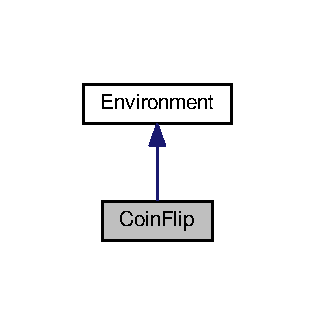
\includegraphics[width=151pt]{class_coin_flip__inherit__graph}
\end{center}
\end{figure}


Collaboration diagram for Coin\+Flip\+:
\nopagebreak
\begin{figure}[H]
\begin{center}
\leavevmode
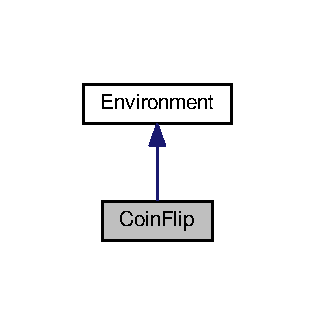
\includegraphics[width=151pt]{class_coin_flip__coll__graph}
\end{center}
\end{figure}
\subsection*{Public Member Functions}
\begin{DoxyCompactItemize}
\item 
{\bf Coin\+Flip} ({\bf options\+\_\+t} \&options)
\item 
virtual void {\bf perform\+Action} ({\bf action\+\_\+t} action)
\end{DoxyCompactItemize}
\subsection*{Additional Inherited Members}


\subsection{Detailed Description}


Definition at line 36 of file environment.\+hpp.



\subsection{Constructor \& Destructor Documentation}
\index{Coin\+Flip@{Coin\+Flip}!Coin\+Flip@{Coin\+Flip}}
\index{Coin\+Flip@{Coin\+Flip}!Coin\+Flip@{Coin\+Flip}}
\subsubsection[{Coin\+Flip}]{\setlength{\rightskip}{0pt plus 5cm}Coin\+Flip\+::\+Coin\+Flip (
\begin{DoxyParamCaption}
\item[{{\bf options\+\_\+t} \&}]{options}
\end{DoxyParamCaption}
)}\label{class_coin_flip_a4ac71bf10be90ec52673c8eaeaa6dff0}


Definition at line 7 of file environment.\+cpp.



\subsection{Member Function Documentation}
\index{Coin\+Flip@{Coin\+Flip}!perform\+Action@{perform\+Action}}
\index{perform\+Action@{perform\+Action}!Coin\+Flip@{Coin\+Flip}}
\subsubsection[{perform\+Action}]{\setlength{\rightskip}{0pt plus 5cm}void Coin\+Flip\+::perform\+Action (
\begin{DoxyParamCaption}
\item[{{\bf action\+\_\+t}}]{action}
\end{DoxyParamCaption}
)\hspace{0.3cm}{\ttfamily [virtual]}}\label{class_coin_flip_a2cdf7d804e5ceb515d45bb4e4f234e93}


Implements {\bf Environment} \doxyref{}{p.}{class_environment_a1686290a116f9a84ee356030ac2eaf96}.



Definition at line 24 of file environment.\+cpp.



The documentation for this class was generated from the following files\+:\begin{DoxyCompactItemize}
\item 
{\bf environment.\+hpp}\item 
{\bf environment.\+cpp}\end{DoxyCompactItemize}

\section{Context\+Tree Class Reference}
\label{class_context_tree}\index{Context\+Tree@{Context\+Tree}}


{\ttfamily \#include $<$predict.\+hpp$>$}

\subsection*{Public Member Functions}
\begin{DoxyCompactItemize}
\item 
{\bf Context\+Tree} (size\+\_\+t {\bf depth})
\item 
{\bf $\sim$\+Context\+Tree} (void)
\item 
void {\bf clear} (void)
\item 
void {\bf update} (const {\bf symbol\+\_\+t} sym)
\item 
void {\bf update} (const {\bf symbol\+\_\+list\+\_\+t} \&symbol\+\_\+list)
\item 
void {\bf update\+History} (const {\bf symbol\+\_\+list\+\_\+t} \&symbol\+\_\+list)
\item 
void {\bf update\+Log\+Probability} (void)
\item 
void {\bf revert} (void)
\item 
void {\bf revert\+History} (size\+\_\+t newsize)
\item 
double {\bf predict} ({\bf symbol\+\_\+t} sym)
\item 
double {\bf predict} ({\bf symbol\+\_\+list\+\_\+t} symbol\+\_\+list)
\item 
void {\bf gen\+Random\+Symbols} ({\bf symbol\+\_\+list\+\_\+t} \&symbols, size\+\_\+t bits)
\item 
void {\bf gen\+Random\+Symbols\+And\+Update} ({\bf symbol\+\_\+list\+\_\+t} \&symbols, size\+\_\+t bits)
\item 
double {\bf log\+Block\+Probability} (void)
\item 
const {\bf symbol\+\_\+t} $\ast$ {\bf nth\+History\+Symbol} (size\+\_\+t n) const 
\item 
size\+\_\+t {\bf depth} (void) const 
\item 
size\+\_\+t {\bf history\+Size} (void) const 
\item 
size\+\_\+t {\bf size} (void) const 
\end{DoxyCompactItemize}


\subsection{Detailed Description}


Definition at line 69 of file predict.\+hpp.



\subsection{Constructor \& Destructor Documentation}
\index{Context\+Tree@{Context\+Tree}!Context\+Tree@{Context\+Tree}}
\index{Context\+Tree@{Context\+Tree}!Context\+Tree@{Context\+Tree}}
\subsubsection[{Context\+Tree}]{\setlength{\rightskip}{0pt plus 5cm}Context\+Tree\+::\+Context\+Tree (
\begin{DoxyParamCaption}
\item[{size\+\_\+t}]{depth}
\end{DoxyParamCaption}
)}\label{class_context_tree_abc815458fcefac810580d9eb3d7831fa}


Definition at line 53 of file predict.\+cpp.

\index{Context\+Tree@{Context\+Tree}!````~Context\+Tree@{$\sim$\+Context\+Tree}}
\index{````~Context\+Tree@{$\sim$\+Context\+Tree}!Context\+Tree@{Context\+Tree}}
\subsubsection[{$\sim$\+Context\+Tree}]{\setlength{\rightskip}{0pt plus 5cm}Context\+Tree\+::$\sim$\+Context\+Tree (
\begin{DoxyParamCaption}
\item[{void}]{}
\end{DoxyParamCaption}
)}\label{class_context_tree_abc17f665f29acb806de3980a4986a30f}


Definition at line 59 of file predict.\+cpp.



\subsection{Member Function Documentation}
\index{Context\+Tree@{Context\+Tree}!clear@{clear}}
\index{clear@{clear}!Context\+Tree@{Context\+Tree}}
\subsubsection[{clear}]{\setlength{\rightskip}{0pt plus 5cm}void Context\+Tree\+::clear (
\begin{DoxyParamCaption}
\item[{void}]{}
\end{DoxyParamCaption}
)}\label{class_context_tree_a0a3c136d70e092fc2251c81e331633f4}


Definition at line 65 of file predict.\+cpp.

\index{Context\+Tree@{Context\+Tree}!depth@{depth}}
\index{depth@{depth}!Context\+Tree@{Context\+Tree}}
\subsubsection[{depth}]{\setlength{\rightskip}{0pt plus 5cm}size\+\_\+t Context\+Tree\+::depth (
\begin{DoxyParamCaption}
\item[{void}]{}
\end{DoxyParamCaption}
) const\hspace{0.3cm}{\ttfamily [inline]}}\label{class_context_tree_a3f77b7ccf862050a37914e559aea94de}


Definition at line 116 of file predict.\+hpp.

\index{Context\+Tree@{Context\+Tree}!gen\+Random\+Symbols@{gen\+Random\+Symbols}}
\index{gen\+Random\+Symbols@{gen\+Random\+Symbols}!Context\+Tree@{Context\+Tree}}
\subsubsection[{gen\+Random\+Symbols}]{\setlength{\rightskip}{0pt plus 5cm}void Context\+Tree\+::gen\+Random\+Symbols (
\begin{DoxyParamCaption}
\item[{{\bf symbol\+\_\+list\+\_\+t} \&}]{symbols, }
\item[{size\+\_\+t}]{bits}
\end{DoxyParamCaption}
)}\label{class_context_tree_a4feda8f2ba7199b99f143a04cf46b761}


Definition at line 108 of file predict.\+cpp.

\index{Context\+Tree@{Context\+Tree}!gen\+Random\+Symbols\+And\+Update@{gen\+Random\+Symbols\+And\+Update}}
\index{gen\+Random\+Symbols\+And\+Update@{gen\+Random\+Symbols\+And\+Update}!Context\+Tree@{Context\+Tree}}
\subsubsection[{gen\+Random\+Symbols\+And\+Update}]{\setlength{\rightskip}{0pt plus 5cm}void Context\+Tree\+::gen\+Random\+Symbols\+And\+Update (
\begin{DoxyParamCaption}
\item[{{\bf symbol\+\_\+list\+\_\+t} \&}]{symbols, }
\item[{size\+\_\+t}]{bits}
\end{DoxyParamCaption}
)}\label{class_context_tree_a6346a099b381623901fc0f3082e70501}


Definition at line 120 of file predict.\+cpp.

\index{Context\+Tree@{Context\+Tree}!history\+Size@{history\+Size}}
\index{history\+Size@{history\+Size}!Context\+Tree@{Context\+Tree}}
\subsubsection[{history\+Size}]{\setlength{\rightskip}{0pt plus 5cm}size\+\_\+t Context\+Tree\+::history\+Size (
\begin{DoxyParamCaption}
\item[{void}]{}
\end{DoxyParamCaption}
) const\hspace{0.3cm}{\ttfamily [inline]}}\label{class_context_tree_a20de2ce4a5380e31e37d772ebba0c063}


Definition at line 119 of file predict.\+hpp.

\index{Context\+Tree@{Context\+Tree}!log\+Block\+Probability@{log\+Block\+Probability}}
\index{log\+Block\+Probability@{log\+Block\+Probability}!Context\+Tree@{Context\+Tree}}
\subsubsection[{log\+Block\+Probability}]{\setlength{\rightskip}{0pt plus 5cm}double Context\+Tree\+::log\+Block\+Probability (
\begin{DoxyParamCaption}
\item[{void}]{}
\end{DoxyParamCaption}
)}\label{class_context_tree_ae81ed9f61cd22890ecf5355283405283}


Definition at line 126 of file predict.\+cpp.

\index{Context\+Tree@{Context\+Tree}!nth\+History\+Symbol@{nth\+History\+Symbol}}
\index{nth\+History\+Symbol@{nth\+History\+Symbol}!Context\+Tree@{Context\+Tree}}
\subsubsection[{nth\+History\+Symbol}]{\setlength{\rightskip}{0pt plus 5cm}const {\bf symbol\+\_\+t} $\ast$ Context\+Tree\+::nth\+History\+Symbol (
\begin{DoxyParamCaption}
\item[{size\+\_\+t}]{n}
\end{DoxyParamCaption}
) const}\label{class_context_tree_a77835b9aa2ff944a3cbe823c6af6a630}


Definition at line 132 of file predict.\+cpp.

\index{Context\+Tree@{Context\+Tree}!predict@{predict}}
\index{predict@{predict}!Context\+Tree@{Context\+Tree}}
\subsubsection[{predict}]{\setlength{\rightskip}{0pt plus 5cm}double Context\+Tree\+::predict (
\begin{DoxyParamCaption}
\item[{{\bf symbol\+\_\+t}}]{sym}
\end{DoxyParamCaption}
)}\label{class_context_tree_aaad4ba47127ef1021090859b5b2e4d07}
\index{Context\+Tree@{Context\+Tree}!predict@{predict}}
\index{predict@{predict}!Context\+Tree@{Context\+Tree}}
\subsubsection[{predict}]{\setlength{\rightskip}{0pt plus 5cm}double Context\+Tree\+::predict (
\begin{DoxyParamCaption}
\item[{{\bf symbol\+\_\+list\+\_\+t}}]{symbol\+\_\+list}
\end{DoxyParamCaption}
)}\label{class_context_tree_afb3c0d7d401009bb5ad57a98f1171a79}
\index{Context\+Tree@{Context\+Tree}!revert@{revert}}
\index{revert@{revert}!Context\+Tree@{Context\+Tree}}
\subsubsection[{revert}]{\setlength{\rightskip}{0pt plus 5cm}void Context\+Tree\+::revert (
\begin{DoxyParamCaption}
\item[{void}]{}
\end{DoxyParamCaption}
)}\label{class_context_tree_a2fc30e6f68a5b1d2df3d5ac786c0d943}


Definition at line 92 of file predict.\+cpp.

\index{Context\+Tree@{Context\+Tree}!revert\+History@{revert\+History}}
\index{revert\+History@{revert\+History}!Context\+Tree@{Context\+Tree}}
\subsubsection[{revert\+History}]{\setlength{\rightskip}{0pt plus 5cm}void Context\+Tree\+::revert\+History (
\begin{DoxyParamCaption}
\item[{size\+\_\+t}]{newsize}
\end{DoxyParamCaption}
)}\label{class_context_tree_adc6eeba995808bfe1bae4e46612cf05b}


Definition at line 98 of file predict.\+cpp.

\index{Context\+Tree@{Context\+Tree}!size@{size}}
\index{size@{size}!Context\+Tree@{Context\+Tree}}
\subsubsection[{size}]{\setlength{\rightskip}{0pt plus 5cm}size\+\_\+t Context\+Tree\+::size (
\begin{DoxyParamCaption}
\item[{void}]{}
\end{DoxyParamCaption}
) const\hspace{0.3cm}{\ttfamily [inline]}}\label{class_context_tree_a2fb583d155c915dd639d78783a3a1711}


Definition at line 122 of file predict.\+hpp.

\index{Context\+Tree@{Context\+Tree}!update@{update}}
\index{update@{update}!Context\+Tree@{Context\+Tree}}
\subsubsection[{update}]{\setlength{\rightskip}{0pt plus 5cm}void Context\+Tree\+::update (
\begin{DoxyParamCaption}
\item[{const {\bf symbol\+\_\+t}}]{sym}
\end{DoxyParamCaption}
)}\label{class_context_tree_a2b06e9c79afec1345a6cc2f86abaa58c}


Definition at line 72 of file predict.\+cpp.

\index{Context\+Tree@{Context\+Tree}!update@{update}}
\index{update@{update}!Context\+Tree@{Context\+Tree}}
\subsubsection[{update}]{\setlength{\rightskip}{0pt plus 5cm}void Context\+Tree\+::update (
\begin{DoxyParamCaption}
\item[{const {\bf symbol\+\_\+list\+\_\+t} \&}]{symbol\+\_\+list}
\end{DoxyParamCaption}
)}\label{class_context_tree_af0a17028f238d31ce3f60bcbbeafa05e}


Definition at line 77 of file predict.\+cpp.

\index{Context\+Tree@{Context\+Tree}!update\+History@{update\+History}}
\index{update\+History@{update\+History}!Context\+Tree@{Context\+Tree}}
\subsubsection[{update\+History}]{\setlength{\rightskip}{0pt plus 5cm}void Context\+Tree\+::update\+History (
\begin{DoxyParamCaption}
\item[{const {\bf symbol\+\_\+list\+\_\+t} \&}]{symbol\+\_\+list}
\end{DoxyParamCaption}
)}\label{class_context_tree_af00a5f156285750c82eee5db34904ada}


Definition at line 83 of file predict.\+cpp.

\index{Context\+Tree@{Context\+Tree}!update\+Log\+Probability@{update\+Log\+Probability}}
\index{update\+Log\+Probability@{update\+Log\+Probability}!Context\+Tree@{Context\+Tree}}
\subsubsection[{update\+Log\+Probability}]{\setlength{\rightskip}{0pt plus 5cm}void Context\+Tree\+::update\+Log\+Probability (
\begin{DoxyParamCaption}
\item[{void}]{}
\end{DoxyParamCaption}
)}\label{class_context_tree_a431c33d37fa23ed3390f1abf20ca2aff}


The documentation for this class was generated from the following files\+:\begin{DoxyCompactItemize}
\item 
{\bf predict.\+hpp}\item 
{\bf predict.\+cpp}\end{DoxyCompactItemize}

\section{C\+T\+Node Class Reference}
\label{class_c_t_node}\index{C\+T\+Node@{C\+T\+Node}}


{\ttfamily \#include $<$predict.\+hpp$>$}

\subsection*{Public Member Functions}
\begin{DoxyCompactItemize}
\item 
{\bf weight\+\_\+t} {\bf log\+Prob\+Weighted} (void) const 
\item 
{\bf weight\+\_\+t} {\bf log\+Prob\+Estimated} (void) const 
\item 
{\bf count\+\_\+t} {\bf visits} (void) const 
\item 
const {\bf C\+T\+Node} $\ast$ {\bf child} ({\bf symbol\+\_\+t} sym) const 
\item 
size\+\_\+t {\bf size} (void) const 
\end{DoxyCompactItemize}
\subsection*{Friends}
\begin{DoxyCompactItemize}
\item 
class {\bf Context\+Tree}
\end{DoxyCompactItemize}


\subsection{Detailed Description}


Definition at line 17 of file predict.\+hpp.



\subsection{Member Function Documentation}
\index{C\+T\+Node@{C\+T\+Node}!child@{child}}
\index{child@{child}!C\+T\+Node@{C\+T\+Node}}
\subsubsection[{child}]{\setlength{\rightskip}{0pt plus 5cm}const {\bf C\+T\+Node}$\ast$ C\+T\+Node\+::child (
\begin{DoxyParamCaption}
\item[{{\bf symbol\+\_\+t}}]{sym}
\end{DoxyParamCaption}
) const\hspace{0.3cm}{\ttfamily [inline]}}\label{class_c_t_node_a82ce7501e56e553538f1a0a49c4c56ae}


Definition at line 31 of file predict.\+hpp.

\index{C\+T\+Node@{C\+T\+Node}!log\+Prob\+Estimated@{log\+Prob\+Estimated}}
\index{log\+Prob\+Estimated@{log\+Prob\+Estimated}!C\+T\+Node@{C\+T\+Node}}
\subsubsection[{log\+Prob\+Estimated}]{\setlength{\rightskip}{0pt plus 5cm}{\bf weight\+\_\+t} C\+T\+Node\+::log\+Prob\+Estimated (
\begin{DoxyParamCaption}
\item[{void}]{}
\end{DoxyParamCaption}
) const\hspace{0.3cm}{\ttfamily [inline]}}\label{class_c_t_node_a4c7150ab370654385667cff00e97c1ff}


Definition at line 25 of file predict.\+hpp.

\index{C\+T\+Node@{C\+T\+Node}!log\+Prob\+Weighted@{log\+Prob\+Weighted}}
\index{log\+Prob\+Weighted@{log\+Prob\+Weighted}!C\+T\+Node@{C\+T\+Node}}
\subsubsection[{log\+Prob\+Weighted}]{\setlength{\rightskip}{0pt plus 5cm}{\bf weight\+\_\+t} C\+T\+Node\+::log\+Prob\+Weighted (
\begin{DoxyParamCaption}
\item[{void}]{}
\end{DoxyParamCaption}
) const\hspace{0.3cm}{\ttfamily [inline]}}\label{class_c_t_node_a2f14dc807c7cc8f706cc0804621f5271}


Definition at line 22 of file predict.\+hpp.

\index{C\+T\+Node@{C\+T\+Node}!size@{size}}
\index{size@{size}!C\+T\+Node@{C\+T\+Node}}
\subsubsection[{size}]{\setlength{\rightskip}{0pt plus 5cm}size\+\_\+t C\+T\+Node\+::size (
\begin{DoxyParamCaption}
\item[{void}]{}
\end{DoxyParamCaption}
) const}\label{class_c_t_node_a52170e90868ce1674dbfa3ab53347161}


Definition at line 24 of file predict.\+cpp.

\index{C\+T\+Node@{C\+T\+Node}!visits@{visits}}
\index{visits@{visits}!C\+T\+Node@{C\+T\+Node}}
\subsubsection[{visits}]{\setlength{\rightskip}{0pt plus 5cm}{\bf count\+\_\+t} C\+T\+Node\+::visits (
\begin{DoxyParamCaption}
\item[{void}]{}
\end{DoxyParamCaption}
) const\hspace{0.3cm}{\ttfamily [inline]}}\label{class_c_t_node_a99231c5c3da67e534f9c844e0cb5a32e}


Definition at line 28 of file predict.\+hpp.



\subsection{Friends And Related Function Documentation}
\index{C\+T\+Node@{C\+T\+Node}!Context\+Tree@{Context\+Tree}}
\index{Context\+Tree@{Context\+Tree}!C\+T\+Node@{C\+T\+Node}}
\subsubsection[{Context\+Tree}]{\setlength{\rightskip}{0pt plus 5cm}friend class {\bf Context\+Tree}\hspace{0.3cm}{\ttfamily [friend]}}\label{class_c_t_node_a6c187d0539879d9c2146538ad4591f84}


Definition at line 18 of file predict.\+hpp.



The documentation for this class was generated from the following files\+:\begin{DoxyCompactItemize}
\item 
{\bf predict.\+hpp}\item 
{\bf predict.\+cpp}\end{DoxyCompactItemize}

\section{Environment Class Reference}
\label{class_environment}\index{Environment@{Environment}}


{\ttfamily \#include $<$environment.\+hpp$>$}



Inheritance diagram for Environment\+:
\nopagebreak
\begin{figure}[H]
\begin{center}
\leavevmode
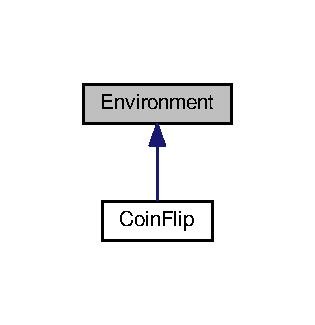
\includegraphics[width=151pt]{class_environment__inherit__graph}
\end{center}
\end{figure}
\subsection*{Public Member Functions}
\begin{DoxyCompactItemize}
\item 
virtual void {\bf perform\+Action} ({\bf action\+\_\+t} action)=0
\item 
virtual bool {\bf is\+Finished} (void) const 
\item 
void {\bf get\+Percept} ({\bf symbol\+\_\+list\+\_\+t} \&symbol\+\_\+list)
\item 
{\bf percept\+\_\+t} {\bf get\+Observation} (void) const 
\item 
{\bf percept\+\_\+t} {\bf get\+Reward} (void) const 
\end{DoxyCompactItemize}
\subsection*{Protected Attributes}
\begin{DoxyCompactItemize}
\item 
{\bf action\+\_\+t} {\bf m\+\_\+last\+\_\+action}
\item 
{\bf percept\+\_\+t} {\bf m\+\_\+observation}
\item 
{\bf percept\+\_\+t} {\bf m\+\_\+reward}
\end{DoxyCompactItemize}


\subsection{Detailed Description}


Definition at line 6 of file environment.\+hpp.



\subsection{Member Function Documentation}
\index{Environment@{Environment}!get\+Observation@{get\+Observation}}
\index{get\+Observation@{get\+Observation}!Environment@{Environment}}
\subsubsection[{get\+Observation}]{\setlength{\rightskip}{0pt plus 5cm}{\bf percept\+\_\+t} Environment\+::get\+Observation (
\begin{DoxyParamCaption}
\item[{void}]{}
\end{DoxyParamCaption}
) const\hspace{0.3cm}{\ttfamily [inline]}}\label{class_environment_a1994d95ea12fe7edc39d55e4e5b08ec2}


Definition at line 21 of file environment.\+hpp.

\index{Environment@{Environment}!get\+Percept@{get\+Percept}}
\index{get\+Percept@{get\+Percept}!Environment@{Environment}}
\subsubsection[{get\+Percept}]{\setlength{\rightskip}{0pt plus 5cm}void Environment\+::get\+Percept (
\begin{DoxyParamCaption}
\item[{{\bf symbol\+\_\+list\+\_\+t} \&}]{symbol\+\_\+list}
\end{DoxyParamCaption}
)}\label{class_environment_a1e488d2d948fd3da1e89e81eaa220e09}
\index{Environment@{Environment}!get\+Reward@{get\+Reward}}
\index{get\+Reward@{get\+Reward}!Environment@{Environment}}
\subsubsection[{get\+Reward}]{\setlength{\rightskip}{0pt plus 5cm}{\bf percept\+\_\+t} Environment\+::get\+Reward (
\begin{DoxyParamCaption}
\item[{void}]{}
\end{DoxyParamCaption}
) const\hspace{0.3cm}{\ttfamily [inline]}}\label{class_environment_a46e81fc25a9aa33f6efce61d44ecadd9}


Definition at line 23 of file environment.\+hpp.

\index{Environment@{Environment}!is\+Finished@{is\+Finished}}
\index{is\+Finished@{is\+Finished}!Environment@{Environment}}
\subsubsection[{is\+Finished}]{\setlength{\rightskip}{0pt plus 5cm}virtual bool Environment\+::is\+Finished (
\begin{DoxyParamCaption}
\item[{void}]{}
\end{DoxyParamCaption}
) const\hspace{0.3cm}{\ttfamily [inline]}, {\ttfamily [virtual]}}\label{class_environment_aa4447dfb59df3df6187cec210f7f5e44}


Definition at line 17 of file environment.\+hpp.

\index{Environment@{Environment}!perform\+Action@{perform\+Action}}
\index{perform\+Action@{perform\+Action}!Environment@{Environment}}
\subsubsection[{perform\+Action}]{\setlength{\rightskip}{0pt plus 5cm}virtual void Environment\+::perform\+Action (
\begin{DoxyParamCaption}
\item[{{\bf action\+\_\+t}}]{action}
\end{DoxyParamCaption}
)\hspace{0.3cm}{\ttfamily [pure virtual]}}\label{class_environment_a1686290a116f9a84ee356030ac2eaf96}


Implemented in {\bf Coin\+Flip} \doxyref{}{p.}{class_coin_flip_a2cdf7d804e5ceb515d45bb4e4f234e93}.



\subsection{Member Data Documentation}
\index{Environment@{Environment}!m\+\_\+last\+\_\+action@{m\+\_\+last\+\_\+action}}
\index{m\+\_\+last\+\_\+action@{m\+\_\+last\+\_\+action}!Environment@{Environment}}
\subsubsection[{m\+\_\+last\+\_\+action}]{\setlength{\rightskip}{0pt plus 5cm}{\bf action\+\_\+t} Environment\+::m\+\_\+last\+\_\+action\hspace{0.3cm}{\ttfamily [protected]}}\label{class_environment_aded1d71d81f4cb1420497c9e8d974f28}


Definition at line 26 of file environment.\+hpp.

\index{Environment@{Environment}!m\+\_\+observation@{m\+\_\+observation}}
\index{m\+\_\+observation@{m\+\_\+observation}!Environment@{Environment}}
\subsubsection[{m\+\_\+observation}]{\setlength{\rightskip}{0pt plus 5cm}{\bf percept\+\_\+t} Environment\+::m\+\_\+observation\hspace{0.3cm}{\ttfamily [protected]}}\label{class_environment_a1bceb1813fe8cdc323430a92728690de}


Definition at line 27 of file environment.\+hpp.

\index{Environment@{Environment}!m\+\_\+reward@{m\+\_\+reward}}
\index{m\+\_\+reward@{m\+\_\+reward}!Environment@{Environment}}
\subsubsection[{m\+\_\+reward}]{\setlength{\rightskip}{0pt plus 5cm}{\bf percept\+\_\+t} Environment\+::m\+\_\+reward\hspace{0.3cm}{\ttfamily [protected]}}\label{class_environment_a6629ea90bd678076e681af5dc973aebd}


Definition at line 28 of file environment.\+hpp.



The documentation for this class was generated from the following file\+:\begin{DoxyCompactItemize}
\item 
{\bf environment.\+hpp}\end{DoxyCompactItemize}

\section{Model\+Undo Class Reference}
\label{class_model_undo}\index{Model\+Undo@{Model\+Undo}}


{\ttfamily \#include $<$agent.\+hpp$>$}

\subsection*{Public Member Functions}
\begin{DoxyCompactItemize}
\item 
{\bf Model\+Undo} (const {\bf Agent} \&agent)
\item 
{\bf lifetime\+\_\+t} {\bf lifetime} (void) const 
\item 
{\bf reward\+\_\+t} {\bf reward} (void) const 
\item 
size\+\_\+t {\bf history\+Size} (void) const 
\item 
bool {\bf last\+Update} (void) const 
\end{DoxyCompactItemize}


\subsection{Detailed Description}


Definition at line 113 of file agent.\+hpp.



\subsection{Constructor \& Destructor Documentation}
\index{Model\+Undo@{Model\+Undo}!Model\+Undo@{Model\+Undo}}
\index{Model\+Undo@{Model\+Undo}!Model\+Undo@{Model\+Undo}}
\subsubsection[{Model\+Undo}]{\setlength{\rightskip}{0pt plus 5cm}Model\+Undo\+::\+Model\+Undo (
\begin{DoxyParamCaption}
\item[{const {\bf Agent} \&}]{agent}
\end{DoxyParamCaption}
)}\label{class_model_undo_ae2cff00dee2642df2e8b8eec21f649e9}


Definition at line 201 of file agent.\+cpp.



\subsection{Member Function Documentation}
\index{Model\+Undo@{Model\+Undo}!history\+Size@{history\+Size}}
\index{history\+Size@{history\+Size}!Model\+Undo@{Model\+Undo}}
\subsubsection[{history\+Size}]{\setlength{\rightskip}{0pt plus 5cm}size\+\_\+t Model\+Undo\+::history\+Size (
\begin{DoxyParamCaption}
\item[{void}]{}
\end{DoxyParamCaption}
) const\hspace{0.3cm}{\ttfamily [inline]}}\label{class_model_undo_ab992dcc54ad74c434a25a821ead50a7a}


Definition at line 126 of file agent.\+hpp.

\index{Model\+Undo@{Model\+Undo}!last\+Update@{last\+Update}}
\index{last\+Update@{last\+Update}!Model\+Undo@{Model\+Undo}}
\subsubsection[{last\+Update}]{\setlength{\rightskip}{0pt plus 5cm}bool Model\+Undo\+::last\+Update (
\begin{DoxyParamCaption}
\item[{void}]{}
\end{DoxyParamCaption}
) const\hspace{0.3cm}{\ttfamily [inline]}}\label{class_model_undo_af9aedad08f191939e3e0ccafaf306625}


Definition at line 128 of file agent.\+hpp.

\index{Model\+Undo@{Model\+Undo}!lifetime@{lifetime}}
\index{lifetime@{lifetime}!Model\+Undo@{Model\+Undo}}
\subsubsection[{lifetime}]{\setlength{\rightskip}{0pt plus 5cm}{\bf lifetime\+\_\+t} Model\+Undo\+::lifetime (
\begin{DoxyParamCaption}
\item[{void}]{}
\end{DoxyParamCaption}
) const\hspace{0.3cm}{\ttfamily [inline]}}\label{class_model_undo_af3dfe21871afc770d96adbf80bb2b58b}


Definition at line 120 of file agent.\+hpp.

\index{Model\+Undo@{Model\+Undo}!reward@{reward}}
\index{reward@{reward}!Model\+Undo@{Model\+Undo}}
\subsubsection[{reward}]{\setlength{\rightskip}{0pt plus 5cm}{\bf reward\+\_\+t} Model\+Undo\+::reward (
\begin{DoxyParamCaption}
\item[{void}]{}
\end{DoxyParamCaption}
) const\hspace{0.3cm}{\ttfamily [inline]}}\label{class_model_undo_a201748cb8c2cbaf13c87cfdd730ffb89}


Definition at line 123 of file agent.\+hpp.



The documentation for this class was generated from the following files\+:\begin{DoxyCompactItemize}
\item 
{\bf agent.\+hpp}\item 
{\bf agent.\+cpp}\end{DoxyCompactItemize}

\section{Search\+Node Class Reference}
\label{class_search_node}\index{Search\+Node@{Search\+Node}}
\subsection*{Public Member Functions}
\begin{DoxyCompactItemize}
\item 
{\bf Search\+Node} (bool is\+\_\+chance\+\_\+node)
\item 
{\bf action\+\_\+t} {\bf select\+Action} ({\bf Agent} \&agent) const 
\item 
{\bf reward\+\_\+t} {\bf expectation} (void) const 
\item 
{\bf reward\+\_\+t} {\bf sample} ({\bf Agent} \&agent, unsigned int dfr)
\item 
{\bf visits\+\_\+t} {\bf visits} (void) const 
\end{DoxyCompactItemize}


\subsection{Detailed Description}


Definition at line 14 of file search.\+cpp.



\subsection{Constructor \& Destructor Documentation}
\index{Search\+Node@{Search\+Node}!Search\+Node@{Search\+Node}}
\index{Search\+Node@{Search\+Node}!Search\+Node@{Search\+Node}}
\subsubsection[{Search\+Node}]{\setlength{\rightskip}{0pt plus 5cm}Search\+Node\+::\+Search\+Node (
\begin{DoxyParamCaption}
\item[{bool}]{is\+\_\+chance\+\_\+node}
\end{DoxyParamCaption}
)}\label{class_search_node_a91e1bb3a58a07cf587a86402b1a0b608}


\subsection{Member Function Documentation}
\index{Search\+Node@{Search\+Node}!expectation@{expectation}}
\index{expectation@{expectation}!Search\+Node@{Search\+Node}}
\subsubsection[{expectation}]{\setlength{\rightskip}{0pt plus 5cm}{\bf reward\+\_\+t} Search\+Node\+::expectation (
\begin{DoxyParamCaption}
\item[{void}]{}
\end{DoxyParamCaption}
) const\hspace{0.3cm}{\ttfamily [inline]}}\label{class_search_node_a346d09705e32a0022746b4a51930f829}


Definition at line 24 of file search.\+cpp.

\index{Search\+Node@{Search\+Node}!sample@{sample}}
\index{sample@{sample}!Search\+Node@{Search\+Node}}
\subsubsection[{sample}]{\setlength{\rightskip}{0pt plus 5cm}{\bf reward\+\_\+t} Search\+Node\+::sample (
\begin{DoxyParamCaption}
\item[{{\bf Agent} \&}]{agent, }
\item[{unsigned int}]{dfr}
\end{DoxyParamCaption}
)}\label{class_search_node_ae1f3e61961a679b12e17a73a74c96c95}
\index{Search\+Node@{Search\+Node}!select\+Action@{select\+Action}}
\index{select\+Action@{select\+Action}!Search\+Node@{Search\+Node}}
\subsubsection[{select\+Action}]{\setlength{\rightskip}{0pt plus 5cm}{\bf action\+\_\+t} Search\+Node\+::select\+Action (
\begin{DoxyParamCaption}
\item[{{\bf Agent} \&}]{agent}
\end{DoxyParamCaption}
) const}\label{class_search_node_abcb771c7cb8581f0d2c8e8fbc6bd9945}
\index{Search\+Node@{Search\+Node}!visits@{visits}}
\index{visits@{visits}!Search\+Node@{Search\+Node}}
\subsubsection[{visits}]{\setlength{\rightskip}{0pt plus 5cm}{\bf visits\+\_\+t} Search\+Node\+::visits (
\begin{DoxyParamCaption}
\item[{void}]{}
\end{DoxyParamCaption}
) const\hspace{0.3cm}{\ttfamily [inline]}}\label{class_search_node_a29b41c78d73bbbf1afe21f709d1b0ff6}


Definition at line 31 of file search.\+cpp.



The documentation for this class was generated from the following file\+:\begin{DoxyCompactItemize}
\item 
{\bf search.\+cpp}\end{DoxyCompactItemize}

\chapter{File Documentation}
\section{agent.\+cpp File Reference}
\label{agent_8cpp}\index{agent.\+cpp@{agent.\+cpp}}
{\ttfamily \#include \char`\"{}agent.\+hpp\char`\"{}}\\*
{\ttfamily \#include $<$cassert$>$}\\*
{\ttfamily \#include \char`\"{}predict.\+hpp\char`\"{}}\\*
{\ttfamily \#include \char`\"{}search.\+hpp\char`\"{}}\\*
{\ttfamily \#include \char`\"{}util.\+hpp\char`\"{}}\\*
Include dependency graph for agent.\+cpp\+:
\nopagebreak
\begin{figure}[H]
\begin{center}
\leavevmode
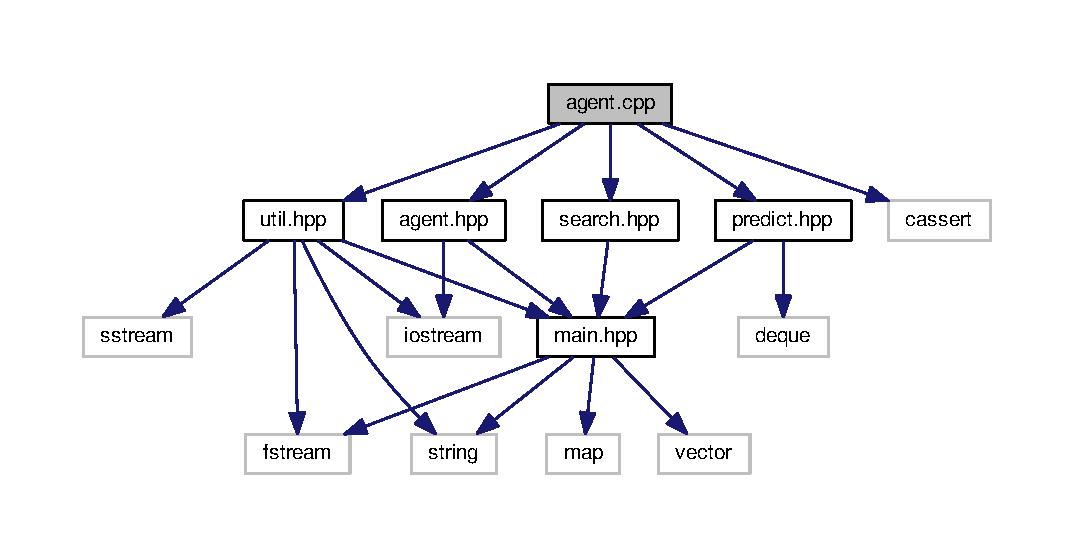
\includegraphics[width=350pt]{agent_8cpp__incl}
\end{center}
\end{figure}

\section{agent.\+hpp File Reference}
\label{agent_8hpp}\index{agent.\+hpp@{agent.\+hpp}}
{\ttfamily \#include $<$iostream$>$}\\*
{\ttfamily \#include \char`\"{}main.\+hpp\char`\"{}}\\*
Include dependency graph for agent.\+hpp\+:
\nopagebreak
\begin{figure}[H]
\begin{center}
\leavevmode
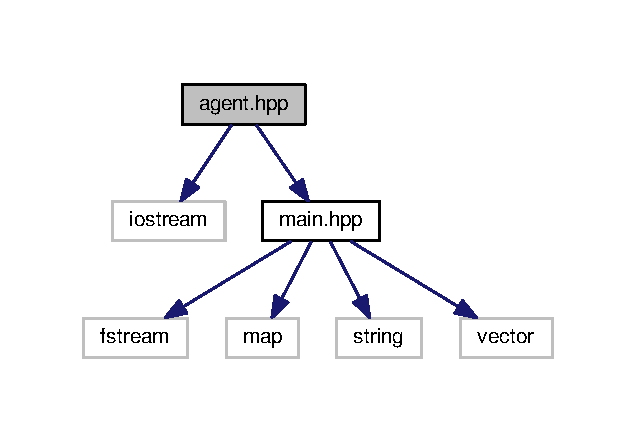
\includegraphics[width=305pt]{agent_8hpp__incl}
\end{center}
\end{figure}
This graph shows which files directly or indirectly include this file\+:
\nopagebreak
\begin{figure}[H]
\begin{center}
\leavevmode
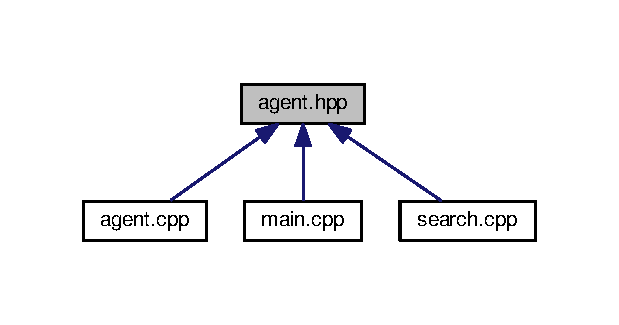
\includegraphics[width=297pt]{agent_8hpp__dep__incl}
\end{center}
\end{figure}
\subsection*{Classes}
\begin{DoxyCompactItemize}
\item 
class {\bf Agent}
\item 
class {\bf Model\+Undo}
\end{DoxyCompactItemize}

\section{environment.\+cpp File Reference}
\label{environment_8cpp}\index{environment.\+cpp@{environment.\+cpp}}
{\ttfamily \#include \char`\"{}environment.\+hpp\char`\"{}}\\*
{\ttfamily \#include $<$cassert$>$}\\*
{\ttfamily \#include \char`\"{}util.\+hpp\char`\"{}}\\*
Include dependency graph for environment.\+cpp\+:
\nopagebreak
\begin{figure}[H]
\begin{center}
\leavevmode
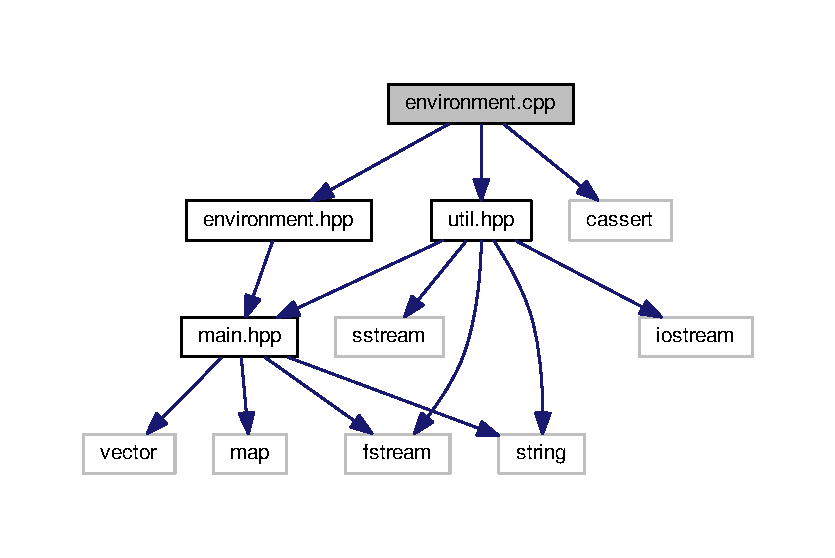
\includegraphics[width=350pt]{environment_8cpp__incl}
\end{center}
\end{figure}

\section{environment.\+hpp File Reference}
\label{environment_8hpp}\index{environment.\+hpp@{environment.\+hpp}}
{\ttfamily \#include \char`\"{}main.\+hpp\char`\"{}}\\*
Include dependency graph for environment.\+hpp\+:
\nopagebreak
\begin{figure}[H]
\begin{center}
\leavevmode
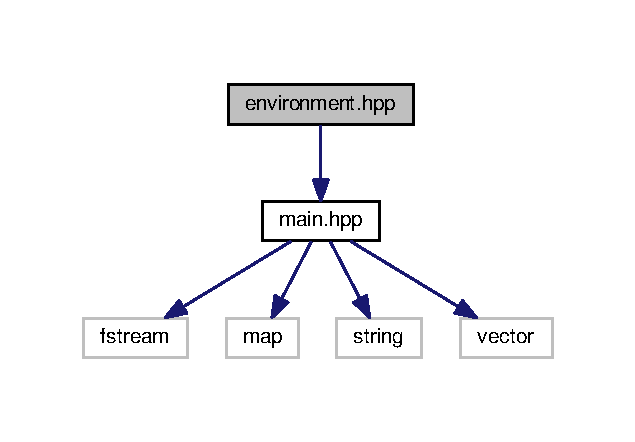
\includegraphics[width=305pt]{environment_8hpp__incl}
\end{center}
\end{figure}
This graph shows which files directly or indirectly include this file\+:
\nopagebreak
\begin{figure}[H]
\begin{center}
\leavevmode
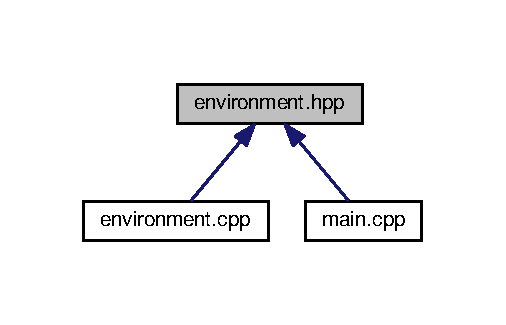
\includegraphics[width=243pt]{environment_8hpp__dep__incl}
\end{center}
\end{figure}
\subsection*{Classes}
\begin{DoxyCompactItemize}
\item 
class {\bf Environment}
\item 
class {\bf Coin\+Flip}
\end{DoxyCompactItemize}

\section{main.\+cpp File Reference}
\label{main_8cpp}\index{main.\+cpp@{main.\+cpp}}
{\ttfamily \#include \char`\"{}main.\+hpp\char`\"{}}\\*
{\ttfamily \#include $<$cassert$>$}\\*
{\ttfamily \#include $<$fstream$>$}\\*
{\ttfamily \#include $<$iostream$>$}\\*
{\ttfamily \#include $<$string$>$}\\*
{\ttfamily \#include \char`\"{}agent.\+hpp\char`\"{}}\\*
{\ttfamily \#include \char`\"{}environment.\+hpp\char`\"{}}\\*
{\ttfamily \#include \char`\"{}search.\+hpp\char`\"{}}\\*
{\ttfamily \#include \char`\"{}util.\+hpp\char`\"{}}\\*
Include dependency graph for main.\+cpp\+:
\nopagebreak
\begin{figure}[H]
\begin{center}
\leavevmode
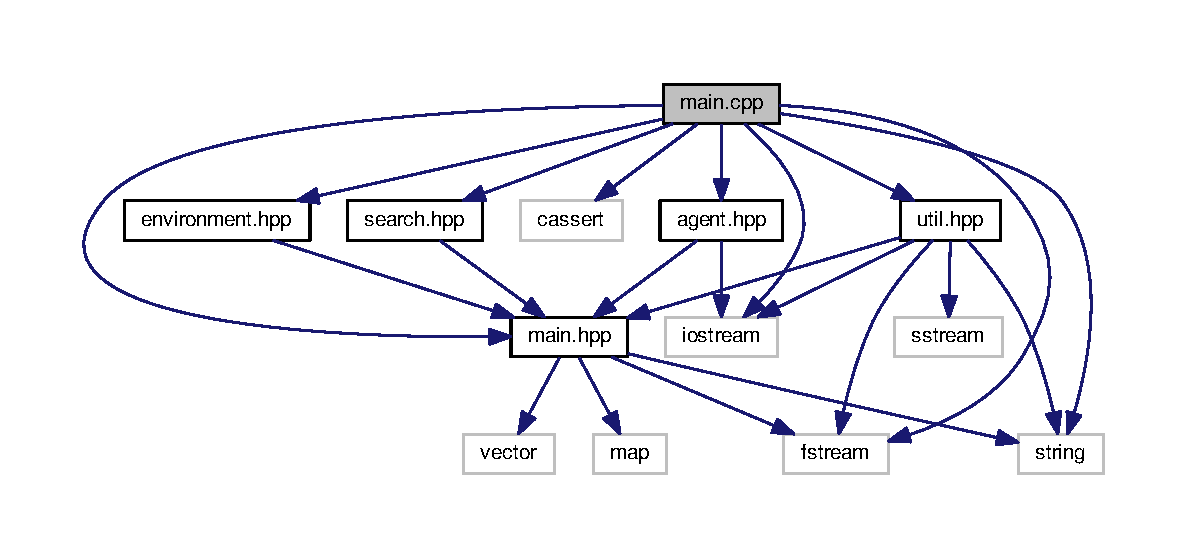
\includegraphics[width=350pt]{main_8cpp__incl}
\end{center}
\end{figure}
\subsection*{Functions}
\begin{DoxyCompactItemize}
\item 
void {\bf main\+Loop} ({\bf Agent} \&ai, {\bf Environment} \&env, {\bf options\+\_\+t} \&options)
\item 
void {\bf process\+Options} (std\+::ifstream \&in, {\bf options\+\_\+t} \&options)
\item 
int {\bf main} (int argc, char $\ast$argv[$\,$])
\end{DoxyCompactItemize}
\subsection*{Variables}
\begin{DoxyCompactItemize}
\item 
std\+::ofstream {\bf log}
\item 
std\+::ofstream {\bf compact\+Log}
\end{DoxyCompactItemize}


\subsection{Function Documentation}
\index{main.\+cpp@{main.\+cpp}!main@{main}}
\index{main@{main}!main.\+cpp@{main.\+cpp}}
\subsubsection[{main}]{\setlength{\rightskip}{0pt plus 5cm}int main (
\begin{DoxyParamCaption}
\item[{int}]{argc, }
\item[{char $\ast$}]{argv[$\,$]}
\end{DoxyParamCaption}
)}\label{main_8cpp_a0ddf1224851353fc92bfbff6f499fa97}


Definition at line 153 of file main.\+cpp.

\index{main.\+cpp@{main.\+cpp}!main\+Loop@{main\+Loop}}
\index{main\+Loop@{main\+Loop}!main.\+cpp@{main.\+cpp}}
\subsubsection[{main\+Loop}]{\setlength{\rightskip}{0pt plus 5cm}void main\+Loop (
\begin{DoxyParamCaption}
\item[{{\bf Agent} \&}]{ai, }
\item[{{\bf Environment} \&}]{env, }
\item[{{\bf options\+\_\+t} \&}]{options}
\end{DoxyParamCaption}
)}\label{main_8cpp_a11389df7ad2551c7378f3912372d3661}


Definition at line 19 of file main.\+cpp.

\index{main.\+cpp@{main.\+cpp}!process\+Options@{process\+Options}}
\index{process\+Options@{process\+Options}!main.\+cpp@{main.\+cpp}}
\subsubsection[{process\+Options}]{\setlength{\rightskip}{0pt plus 5cm}void process\+Options (
\begin{DoxyParamCaption}
\item[{std\+::ifstream \&}]{in, }
\item[{{\bf options\+\_\+t} \&}]{options}
\end{DoxyParamCaption}
)}\label{main_8cpp_acbf464bdc1c8e1dfe2ee5f44abe0d40c}


Definition at line 110 of file main.\+cpp.



\subsection{Variable Documentation}
\index{main.\+cpp@{main.\+cpp}!compact\+Log@{compact\+Log}}
\index{compact\+Log@{compact\+Log}!main.\+cpp@{main.\+cpp}}
\subsubsection[{compact\+Log}]{\setlength{\rightskip}{0pt plus 5cm}std\+::ofstream compact\+Log}\label{main_8cpp_aea45ea491228e65ad5260c65e592e801}


Definition at line 16 of file main.\+cpp.

\index{main.\+cpp@{main.\+cpp}!log@{log}}
\index{log@{log}!main.\+cpp@{main.\+cpp}}
\subsubsection[{log}]{\setlength{\rightskip}{0pt plus 5cm}std\+::ofstream log}\label{main_8cpp_a32def6abcbf45dc4ffc6bf743fc9bb61}


Definition at line 15 of file main.\+cpp.


\section{main.\+hpp File Reference}
\label{main_8hpp}\index{main.\+hpp@{main.\+hpp}}
{\ttfamily \#include $<$fstream$>$}\\*
{\ttfamily \#include $<$map$>$}\\*
{\ttfamily \#include $<$string$>$}\\*
{\ttfamily \#include $<$vector$>$}\\*
Include dependency graph for main.\+hpp\+:
\nopagebreak
\begin{figure}[H]
\begin{center}
\leavevmode
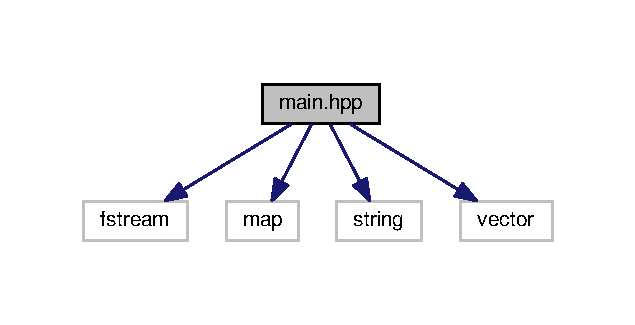
\includegraphics[width=305pt]{main_8hpp__incl}
\end{center}
\end{figure}
This graph shows which files directly or indirectly include this file\+:
\nopagebreak
\begin{figure}[H]
\begin{center}
\leavevmode
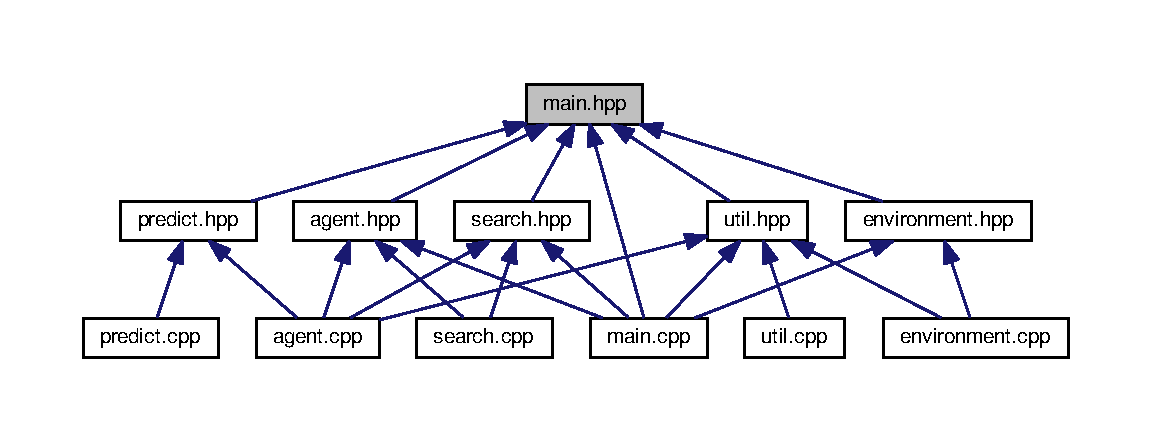
\includegraphics[width=350pt]{main_8hpp__dep__incl}
\end{center}
\end{figure}
\subsection*{Typedefs}
\begin{DoxyCompactItemize}
\item 
typedef bool {\bf symbol\+\_\+t}
\item 
typedef std\+::vector$<$ {\bf symbol\+\_\+t} $>$ {\bf symbol\+\_\+list\+\_\+t}
\item 
typedef double {\bf reward\+\_\+t}
\item 
typedef unsigned int {\bf percept\+\_\+t}
\item 
typedef unsigned long long {\bf lifetime\+\_\+t}
\item 
typedef unsigned int {\bf action\+\_\+t}
\item 
typedef std\+::map$<$ std\+::string, std\+::string $>$ {\bf options\+\_\+t}
\end{DoxyCompactItemize}
\subsection*{Variables}
\begin{DoxyCompactItemize}
\item 
std\+::ofstream {\bf log}
\item 
std\+::ofstream {\bf compact\+Log}
\end{DoxyCompactItemize}


\subsection{Typedef Documentation}
\index{main.\+hpp@{main.\+hpp}!action\+\_\+t@{action\+\_\+t}}
\index{action\+\_\+t@{action\+\_\+t}!main.\+hpp@{main.\+hpp}}
\subsubsection[{action\+\_\+t}]{\setlength{\rightskip}{0pt plus 5cm}typedef unsigned int {\bf action\+\_\+t}}\label{main_8hpp_aa34a2cbe4c2a981beb51a5e6e625037a}


Definition at line 29 of file main.\+hpp.

\index{main.\+hpp@{main.\+hpp}!lifetime\+\_\+t@{lifetime\+\_\+t}}
\index{lifetime\+\_\+t@{lifetime\+\_\+t}!main.\+hpp@{main.\+hpp}}
\subsubsection[{lifetime\+\_\+t}]{\setlength{\rightskip}{0pt plus 5cm}typedef unsigned long long {\bf lifetime\+\_\+t}}\label{main_8hpp_a833e74b5bb1ab434077c5b068671e4b1}


Definition at line 26 of file main.\+hpp.

\index{main.\+hpp@{main.\+hpp}!options\+\_\+t@{options\+\_\+t}}
\index{options\+\_\+t@{options\+\_\+t}!main.\+hpp@{main.\+hpp}}
\subsubsection[{options\+\_\+t}]{\setlength{\rightskip}{0pt plus 5cm}typedef std\+::map$<$std\+::string, std\+::string$>$ {\bf options\+\_\+t}}\label{main_8hpp_a0ff5cac1a4007bb330b7d9939650c283}


Definition at line 32 of file main.\+hpp.

\index{main.\+hpp@{main.\+hpp}!percept\+\_\+t@{percept\+\_\+t}}
\index{percept\+\_\+t@{percept\+\_\+t}!main.\+hpp@{main.\+hpp}}
\subsubsection[{percept\+\_\+t}]{\setlength{\rightskip}{0pt plus 5cm}typedef unsigned int {\bf percept\+\_\+t}}\label{main_8hpp_a6be73834eb109c1d8bb86b99f4dc7e16}


Definition at line 23 of file main.\+hpp.

\index{main.\+hpp@{main.\+hpp}!reward\+\_\+t@{reward\+\_\+t}}
\index{reward\+\_\+t@{reward\+\_\+t}!main.\+hpp@{main.\+hpp}}
\subsubsection[{reward\+\_\+t}]{\setlength{\rightskip}{0pt plus 5cm}typedef double {\bf reward\+\_\+t}}\label{main_8hpp_a008010a51f193f33b2e94c75e10d30b2}


Definition at line 20 of file main.\+hpp.

\index{main.\+hpp@{main.\+hpp}!symbol\+\_\+list\+\_\+t@{symbol\+\_\+list\+\_\+t}}
\index{symbol\+\_\+list\+\_\+t@{symbol\+\_\+list\+\_\+t}!main.\+hpp@{main.\+hpp}}
\subsubsection[{symbol\+\_\+list\+\_\+t}]{\setlength{\rightskip}{0pt plus 5cm}typedef std\+::vector$<${\bf symbol\+\_\+t}$>$ {\bf symbol\+\_\+list\+\_\+t}}\label{main_8hpp_a96913eb6aee99146c546467f52cf18dc}


Definition at line 17 of file main.\+hpp.

\index{main.\+hpp@{main.\+hpp}!symbol\+\_\+t@{symbol\+\_\+t}}
\index{symbol\+\_\+t@{symbol\+\_\+t}!main.\+hpp@{main.\+hpp}}
\subsubsection[{symbol\+\_\+t}]{\setlength{\rightskip}{0pt plus 5cm}typedef bool {\bf symbol\+\_\+t}}\label{main_8hpp_a9b3af827bd2e8ad5d4d0d36c6ef7e897}


Definition at line 14 of file main.\+hpp.



\subsection{Variable Documentation}
\index{main.\+hpp@{main.\+hpp}!compact\+Log@{compact\+Log}}
\index{compact\+Log@{compact\+Log}!main.\+hpp@{main.\+hpp}}
\subsubsection[{compact\+Log}]{\setlength{\rightskip}{0pt plus 5cm}std\+::ofstream compact\+Log}\label{main_8hpp_aea45ea491228e65ad5260c65e592e801}


Definition at line 16 of file main.\+cpp.

\index{main.\+hpp@{main.\+hpp}!log@{log}}
\index{log@{log}!main.\+hpp@{main.\+hpp}}
\subsubsection[{log}]{\setlength{\rightskip}{0pt plus 5cm}std\+::ofstream log}\label{main_8hpp_a32def6abcbf45dc4ffc6bf743fc9bb61}


Definition at line 15 of file main.\+cpp.


\section{predict.\+cpp File Reference}
\label{predict_8cpp}\index{predict.\+cpp@{predict.\+cpp}}
{\ttfamily \#include \char`\"{}predict.\+hpp\char`\"{}}\\*
{\ttfamily \#include $<$cassert$>$}\\*
Include dependency graph for predict.\+cpp\+:
\nopagebreak
\begin{figure}[H]
\begin{center}
\leavevmode
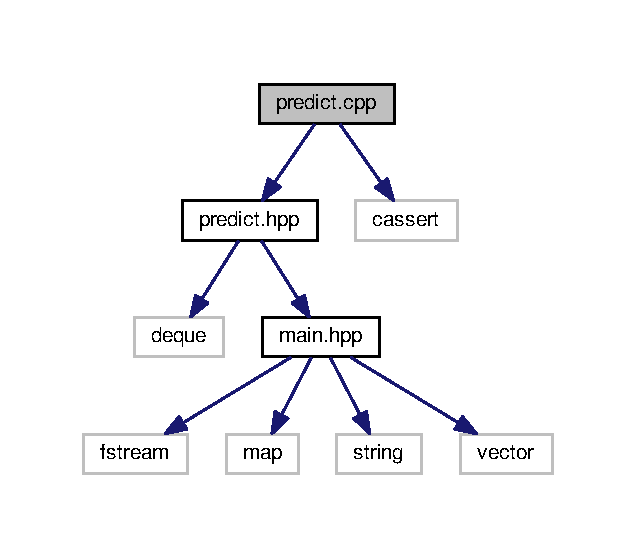
\includegraphics[width=305pt]{predict_8cpp__incl}
\end{center}
\end{figure}

\section{predict.\+hpp File Reference}
\label{predict_8hpp}\index{predict.\+hpp@{predict.\+hpp}}
{\ttfamily \#include $<$deque$>$}\\*
{\ttfamily \#include \char`\"{}main.\+hpp\char`\"{}}\\*
Include dependency graph for predict.\+hpp\+:
\nopagebreak
\begin{figure}[H]
\begin{center}
\leavevmode
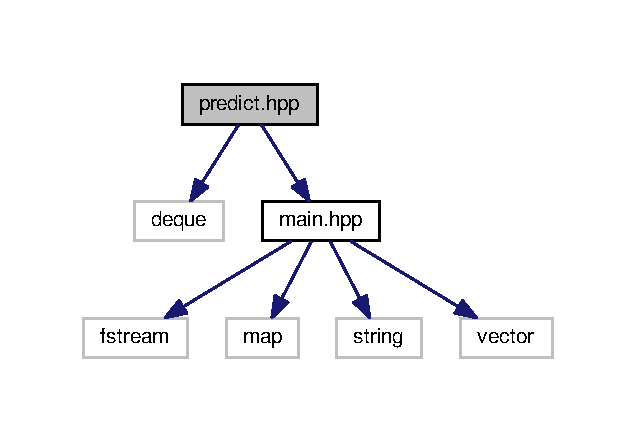
\includegraphics[width=305pt]{predict_8hpp__incl}
\end{center}
\end{figure}
This graph shows which files directly or indirectly include this file\+:
\nopagebreak
\begin{figure}[H]
\begin{center}
\leavevmode
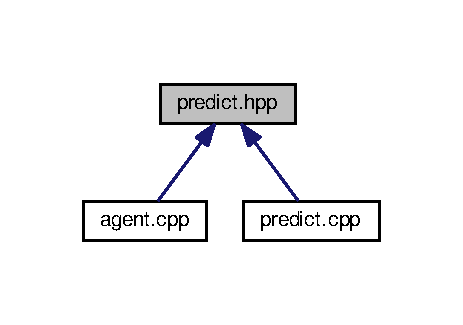
\includegraphics[width=222pt]{predict_8hpp__dep__incl}
\end{center}
\end{figure}
\subsection*{Classes}
\begin{DoxyCompactItemize}
\item 
class {\bf C\+T\+Node}
\item 
class {\bf Context\+Tree}
\end{DoxyCompactItemize}
\subsection*{Typedefs}
\begin{DoxyCompactItemize}
\item 
typedef unsigned int {\bf count\+\_\+t}
\item 
typedef double {\bf weight\+\_\+t}
\item 
typedef std\+::deque$<$ {\bf symbol\+\_\+t} $>$ {\bf history\+\_\+t}
\end{DoxyCompactItemize}


\subsection{Typedef Documentation}
\index{predict.\+hpp@{predict.\+hpp}!count\+\_\+t@{count\+\_\+t}}
\index{count\+\_\+t@{count\+\_\+t}!predict.\+hpp@{predict.\+hpp}}
\subsubsection[{count\+\_\+t}]{\setlength{\rightskip}{0pt plus 5cm}typedef unsigned int {\bf count\+\_\+t}}\label{predict_8hpp_a16e0562e486ffc952cb8f7ca8eefe205}


Definition at line 9 of file predict.\+hpp.

\index{predict.\+hpp@{predict.\+hpp}!history\+\_\+t@{history\+\_\+t}}
\index{history\+\_\+t@{history\+\_\+t}!predict.\+hpp@{predict.\+hpp}}
\subsubsection[{history\+\_\+t}]{\setlength{\rightskip}{0pt plus 5cm}typedef std\+::deque$<${\bf symbol\+\_\+t}$>$ {\bf history\+\_\+t}}\label{predict_8hpp_a5b32b228df5bc910d9bfe7a0310828e5}


Definition at line 15 of file predict.\+hpp.

\index{predict.\+hpp@{predict.\+hpp}!weight\+\_\+t@{weight\+\_\+t}}
\index{weight\+\_\+t@{weight\+\_\+t}!predict.\+hpp@{predict.\+hpp}}
\subsubsection[{weight\+\_\+t}]{\setlength{\rightskip}{0pt plus 5cm}typedef double {\bf weight\+\_\+t}}\label{predict_8hpp_ac7889bf9b3596f63c57011af217212dd}


Definition at line 12 of file predict.\+hpp.


\section{search.\+cpp File Reference}
\label{search_8cpp}\index{search.\+cpp@{search.\+cpp}}
{\ttfamily \#include \char`\"{}search.\+hpp\char`\"{}}\\*
{\ttfamily \#include \char`\"{}agent.\+hpp\char`\"{}}\\*
Include dependency graph for search.\+cpp\+:
\nopagebreak
\begin{figure}[H]
\begin{center}
\leavevmode
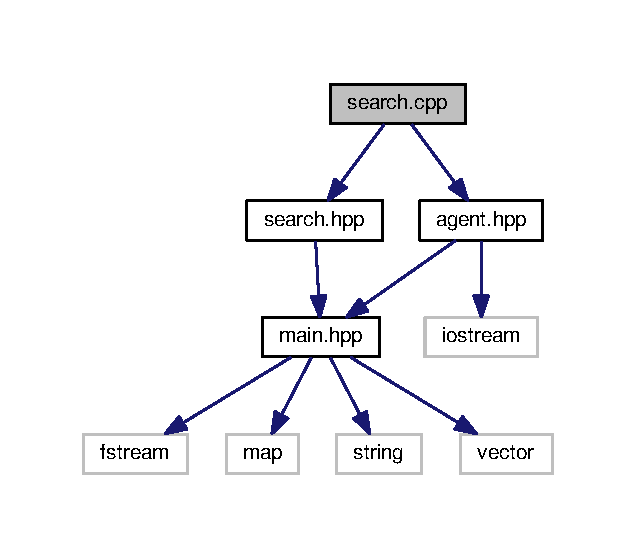
\includegraphics[width=305pt]{search_8cpp__incl}
\end{center}
\end{figure}
\subsection*{Classes}
\begin{DoxyCompactItemize}
\item 
class {\bf Search\+Node}
\end{DoxyCompactItemize}
\subsection*{Typedefs}
\begin{DoxyCompactItemize}
\item 
typedef unsigned long long {\bf visits\+\_\+t}
\end{DoxyCompactItemize}
\subsection*{Functions}
\begin{DoxyCompactItemize}
\item 
{\bf action\+\_\+t} {\bf search} ({\bf Agent} \&agent)
\end{DoxyCompactItemize}


\subsection{Typedef Documentation}
\index{search.\+cpp@{search.\+cpp}!visits\+\_\+t@{visits\+\_\+t}}
\index{visits\+\_\+t@{visits\+\_\+t}!search.\+cpp@{search.\+cpp}}
\subsubsection[{visits\+\_\+t}]{\setlength{\rightskip}{0pt plus 5cm}typedef unsigned long long {\bf visits\+\_\+t}}\label{search_8cpp_a9aad7ec95a808df753c8ea4a0dbc2c35}


Definition at line 5 of file search.\+cpp.



\subsection{Function Documentation}
\index{search.\+cpp@{search.\+cpp}!search@{search}}
\index{search@{search}!search.\+cpp@{search.\+cpp}}
\subsubsection[{search}]{\setlength{\rightskip}{0pt plus 5cm}{\bf action\+\_\+t} search (
\begin{DoxyParamCaption}
\item[{{\bf Agent} \&}]{agent}
\end{DoxyParamCaption}
)}\label{search_8cpp_a1ddcdaabfa488e35e4057ba26ea838ce}


Definition at line 50 of file search.\+cpp.


\section{search.\+hpp File Reference}
\label{search_8hpp}\index{search.\+hpp@{search.\+hpp}}
{\ttfamily \#include \char`\"{}main.\+hpp\char`\"{}}\\*
Include dependency graph for search.\+hpp\+:
\nopagebreak
\begin{figure}[H]
\begin{center}
\leavevmode
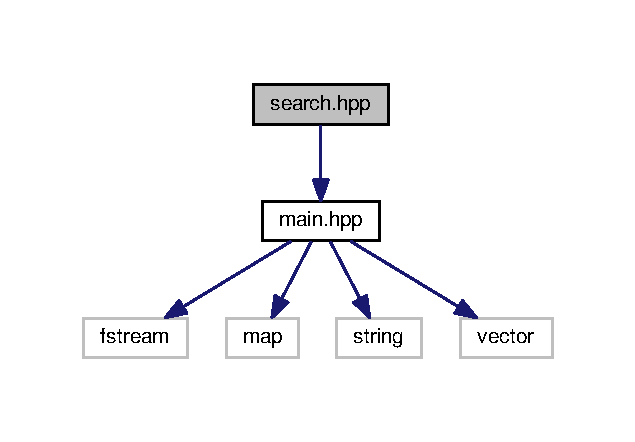
\includegraphics[width=305pt]{search_8hpp__incl}
\end{center}
\end{figure}
This graph shows which files directly or indirectly include this file\+:
\nopagebreak
\begin{figure}[H]
\begin{center}
\leavevmode
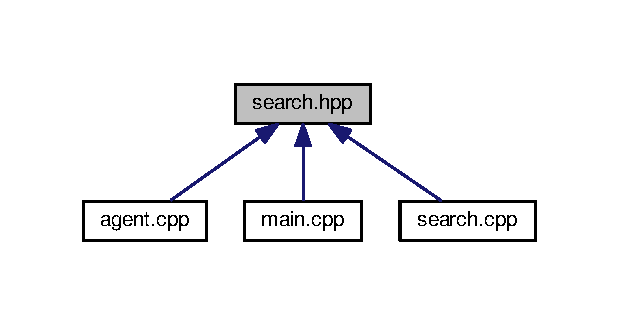
\includegraphics[width=297pt]{search_8hpp__dep__incl}
\end{center}
\end{figure}
\subsection*{Functions}
\begin{DoxyCompactItemize}
\item 
{\bf action\+\_\+t} {\bf search} ({\bf Agent} \&agent)
\end{DoxyCompactItemize}


\subsection{Function Documentation}
\index{search.\+hpp@{search.\+hpp}!search@{search}}
\index{search@{search}!search.\+hpp@{search.\+hpp}}
\subsubsection[{search}]{\setlength{\rightskip}{0pt plus 5cm}{\bf action\+\_\+t} search (
\begin{DoxyParamCaption}
\item[{{\bf Agent} \&}]{agent}
\end{DoxyParamCaption}
)}\label{search_8hpp_a1ddcdaabfa488e35e4057ba26ea838ce}


Definition at line 50 of file search.\+cpp.


\section{util.\+cpp File Reference}
\label{util_8cpp}\index{util.\+cpp@{util.\+cpp}}
{\ttfamily \#include \char`\"{}util.\+hpp\char`\"{}}\\*
{\ttfamily \#include $<$cassert$>$}\\*
{\ttfamily \#include $<$cstdlib$>$}\\*
Include dependency graph for util.\+cpp\+:
\nopagebreak
\begin{figure}[H]
\begin{center}
\leavevmode
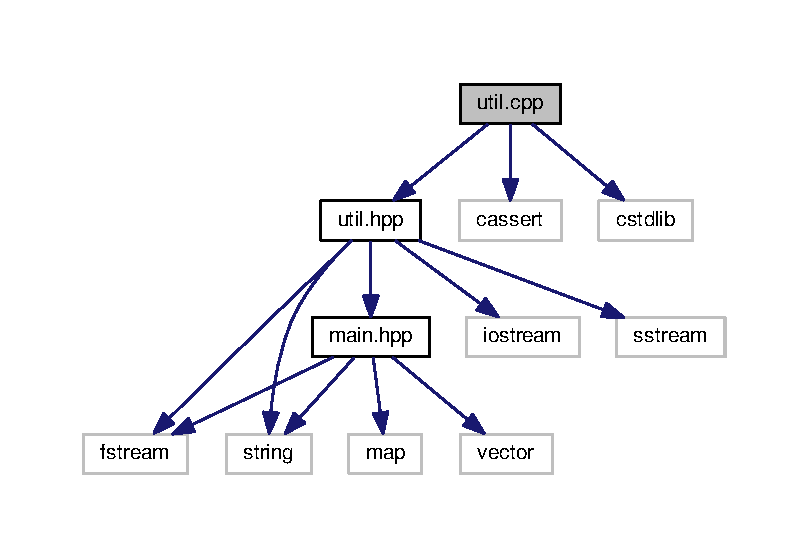
\includegraphics[width=350pt]{util_8cpp__incl}
\end{center}
\end{figure}
\subsection*{Functions}
\begin{DoxyCompactItemize}
\item 
double {\bf rand01} ()
\item 
unsigned int {\bf rand\+Range} (unsigned int end)
\item 
int {\bf rand\+Range} (int start, int end)
\item 
unsigned int {\bf decode} (const {\bf symbol\+\_\+list\+\_\+t} \&symlist, unsigned int bits)
\item 
void {\bf encode} ({\bf symbol\+\_\+list\+\_\+t} \&symlist, unsigned int value, unsigned int bits)
\end{DoxyCompactItemize}


\subsection{Function Documentation}
\index{util.\+cpp@{util.\+cpp}!decode@{decode}}
\index{decode@{decode}!util.\+cpp@{util.\+cpp}}
\subsubsection[{decode}]{\setlength{\rightskip}{0pt plus 5cm}unsigned int decode (
\begin{DoxyParamCaption}
\item[{const {\bf symbol\+\_\+list\+\_\+t} \&}]{symlist, }
\item[{unsigned int}]{bits}
\end{DoxyParamCaption}
)}\label{util_8cpp_aee63a302197282df8a64ef22d45329ba}


Definition at line 31 of file util.\+cpp.

\index{util.\+cpp@{util.\+cpp}!encode@{encode}}
\index{encode@{encode}!util.\+cpp@{util.\+cpp}}
\subsubsection[{encode}]{\setlength{\rightskip}{0pt plus 5cm}void encode (
\begin{DoxyParamCaption}
\item[{{\bf symbol\+\_\+list\+\_\+t} \&}]{symlist, }
\item[{unsigned int}]{value, }
\item[{unsigned int}]{bits}
\end{DoxyParamCaption}
)}\label{util_8cpp_aba6da77df3b0fd3edad6f454732d7d21}


Definition at line 46 of file util.\+cpp.

\index{util.\+cpp@{util.\+cpp}!rand01@{rand01}}
\index{rand01@{rand01}!util.\+cpp@{util.\+cpp}}
\subsubsection[{rand01}]{\setlength{\rightskip}{0pt plus 5cm}double rand01 (
\begin{DoxyParamCaption}
{}
\end{DoxyParamCaption}
)}\label{util_8cpp_afcdd36ac06c749108e82f60508115f36}


Definition at line 8 of file util.\+cpp.

\index{util.\+cpp@{util.\+cpp}!rand\+Range@{rand\+Range}}
\index{rand\+Range@{rand\+Range}!util.\+cpp@{util.\+cpp}}
\subsubsection[{rand\+Range}]{\setlength{\rightskip}{0pt plus 5cm}unsigned int rand\+Range (
\begin{DoxyParamCaption}
\item[{unsigned int}]{end}
\end{DoxyParamCaption}
)}\label{util_8cpp_abc56db15d93d5a6efdffd874e478e1a7}


Definition at line 13 of file util.\+cpp.

\index{util.\+cpp@{util.\+cpp}!rand\+Range@{rand\+Range}}
\index{rand\+Range@{rand\+Range}!util.\+cpp@{util.\+cpp}}
\subsubsection[{rand\+Range}]{\setlength{\rightskip}{0pt plus 5cm}int rand\+Range (
\begin{DoxyParamCaption}
\item[{int}]{start, }
\item[{int}]{end}
\end{DoxyParamCaption}
)}\label{util_8cpp_a3a76408a2c720e5f95cdf70be23b3c55}


Definition at line 24 of file util.\+cpp.


\section{util.\+hpp File Reference}
\label{util_8hpp}\index{util.\+hpp@{util.\+hpp}}
{\ttfamily \#include $<$fstream$>$}\\*
{\ttfamily \#include $<$iostream$>$}\\*
{\ttfamily \#include $<$sstream$>$}\\*
{\ttfamily \#include $<$string$>$}\\*
{\ttfamily \#include \char`\"{}main.\+hpp\char`\"{}}\\*
Include dependency graph for util.\+hpp\+:
\nopagebreak
\begin{figure}[H]
\begin{center}
\leavevmode
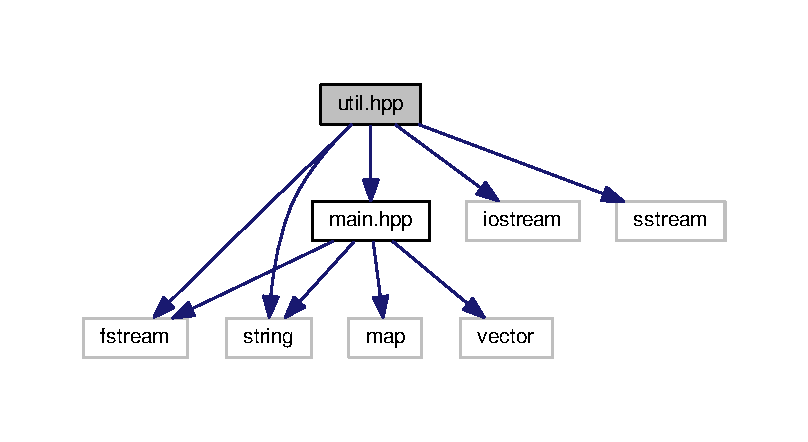
\includegraphics[width=350pt]{util_8hpp__incl}
\end{center}
\end{figure}
This graph shows which files directly or indirectly include this file\+:
\nopagebreak
\begin{figure}[H]
\begin{center}
\leavevmode
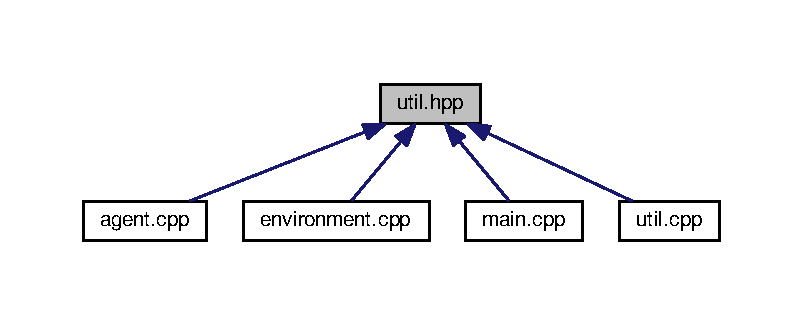
\includegraphics[width=350pt]{util_8hpp__dep__incl}
\end{center}
\end{figure}
\subsection*{Functions}
\begin{DoxyCompactItemize}
\item 
double {\bf rand01} ()
\item 
unsigned int {\bf rand\+Range} (unsigned int end)
\item 
int {\bf rand\+Range} (int start, int end)
\item 
{\footnotesize template$<$typename T $>$ }\\void {\bf str\+Extract} (std\+::string \&str, T \&val)
\item 
{\footnotesize template$<$typename T $>$ }\\T {\bf str\+Extract} (std\+::string \&str)
\item 
unsigned int {\bf decode} (const {\bf symbol\+\_\+list\+\_\+t} \&symlist, unsigned int bits)
\item 
void {\bf encode} ({\bf symbol\+\_\+list\+\_\+t} \&symlist, unsigned int value, unsigned int bits)
\end{DoxyCompactItemize}


\subsection{Function Documentation}
\index{util.\+hpp@{util.\+hpp}!decode@{decode}}
\index{decode@{decode}!util.\+hpp@{util.\+hpp}}
\subsubsection[{decode}]{\setlength{\rightskip}{0pt plus 5cm}unsigned int decode (
\begin{DoxyParamCaption}
\item[{const {\bf symbol\+\_\+list\+\_\+t} \&}]{symlist, }
\item[{unsigned int}]{bits}
\end{DoxyParamCaption}
)}\label{util_8hpp_aee63a302197282df8a64ef22d45329ba}


Definition at line 31 of file util.\+cpp.

\index{util.\+hpp@{util.\+hpp}!encode@{encode}}
\index{encode@{encode}!util.\+hpp@{util.\+hpp}}
\subsubsection[{encode}]{\setlength{\rightskip}{0pt plus 5cm}void encode (
\begin{DoxyParamCaption}
\item[{{\bf symbol\+\_\+list\+\_\+t} \&}]{symlist, }
\item[{unsigned int}]{value, }
\item[{unsigned int}]{bits}
\end{DoxyParamCaption}
)}\label{util_8hpp_aba6da77df3b0fd3edad6f454732d7d21}


Definition at line 46 of file util.\+cpp.

\index{util.\+hpp@{util.\+hpp}!rand01@{rand01}}
\index{rand01@{rand01}!util.\+hpp@{util.\+hpp}}
\subsubsection[{rand01}]{\setlength{\rightskip}{0pt plus 5cm}double rand01 (
\begin{DoxyParamCaption}
{}
\end{DoxyParamCaption}
)}\label{util_8hpp_afcdd36ac06c749108e82f60508115f36}


Definition at line 8 of file util.\+cpp.

\index{util.\+hpp@{util.\+hpp}!rand\+Range@{rand\+Range}}
\index{rand\+Range@{rand\+Range}!util.\+hpp@{util.\+hpp}}
\subsubsection[{rand\+Range}]{\setlength{\rightskip}{0pt plus 5cm}unsigned int rand\+Range (
\begin{DoxyParamCaption}
\item[{unsigned int}]{end}
\end{DoxyParamCaption}
)}\label{util_8hpp_abc56db15d93d5a6efdffd874e478e1a7}


Definition at line 13 of file util.\+cpp.

\index{util.\+hpp@{util.\+hpp}!rand\+Range@{rand\+Range}}
\index{rand\+Range@{rand\+Range}!util.\+hpp@{util.\+hpp}}
\subsubsection[{rand\+Range}]{\setlength{\rightskip}{0pt plus 5cm}int rand\+Range (
\begin{DoxyParamCaption}
\item[{int}]{start, }
\item[{int}]{end}
\end{DoxyParamCaption}
)}\label{util_8hpp_a3a76408a2c720e5f95cdf70be23b3c55}


Definition at line 24 of file util.\+cpp.

\index{util.\+hpp@{util.\+hpp}!str\+Extract@{str\+Extract}}
\index{str\+Extract@{str\+Extract}!util.\+hpp@{util.\+hpp}}
\subsubsection[{str\+Extract}]{\setlength{\rightskip}{0pt plus 5cm}template$<$typename T $>$ void str\+Extract (
\begin{DoxyParamCaption}
\item[{std\+::string \&}]{str, }
\item[{T \&}]{val}
\end{DoxyParamCaption}
)}\label{util_8hpp_a3383816b8869c650b81fbf259ecc783e}


Definition at line 22 of file util.\+hpp.

\index{util.\+hpp@{util.\+hpp}!str\+Extract@{str\+Extract}}
\index{str\+Extract@{str\+Extract}!util.\+hpp@{util.\+hpp}}
\subsubsection[{str\+Extract}]{\setlength{\rightskip}{0pt plus 5cm}template$<$typename T $>$ T str\+Extract (
\begin{DoxyParamCaption}
\item[{std\+::string \&}]{str}
\end{DoxyParamCaption}
)}\label{util_8hpp_a25a8eb09136f99e9c2a660a8d8996972}


Definition at line 28 of file util.\+hpp.


%--- End generated contents ---

% Index
\backmatter
\newpage
\phantomsection
\clearemptydoublepage
\addcontentsline{toc}{chapter}{Index}
\printindex

\end{document}
